\documentclass[conference]{IEEEtran}
\usepackage{microtype,mathtools,amsmath,multibib,amsfonts,multicol,array,multirow,place ins,cite,balance,makecell,algorithm,algorithmic,subfigure,paralist}
%\usepackage{flushend}
\usepackage{graphicx}
\usepackage{listings}
\usepackage{url}
\usepackage[font=small,labelfont=bf]{caption}

\usepackage{xspace}
\usepackage{color}
\usepackage{ifthen}
\usepackage{fancybox}


\graphicspath{{zu/}}
\DeclareGraphicsExtensions{.pdf,.jpeg,.png}
\hyphenation{op-tical net-works semi-conduc-tor}


\begin{document}
\title{ {\Large Less than a week left, still without a}\\ Title}

\author{
\IEEEauthorblockN{Thai Pangsakulyanont\IEEEauthorrefmark{1}, Patanamon Thongtanunam\IEEEauthorrefmark{2},  Daniel Port\IEEEauthorrefmark{3}, Hajimu Iida\IEEEauthorrefmark{2}}
\\
\IEEEauthorblockA{
\IEEEauthorrefmark{1} Kasetsart University, Thailand\\
b5410545036@ku.ac.th
}

\IEEEauthorblockA{
\IEEEauthorrefmark{2} Nara Institute of Science and Technology, Japan\\
patanamon-t@is.naist.jp, iida@itc.naist.jp\\
}

\IEEEauthorblockA{
\IEEEauthorrefmark{3} University of Hawaii at Manoa, USA\\
dport@hawaii.edu \\
}
}


\maketitle
\newboolean{showcomments}
\setboolean{showcomments}{true} % toggle to show or hide comments
\ifthenelse{\boolean{showcomments}}
{\newcommand{\nbnote}[2]{
  % \fbox{\bfseries\sffamily\scriptsize#1}
  \fcolorbox{blue}{yellow}{\bfseries\sffamily\scriptsize#1}
  {\sf\small\textit{#2}}
  % \marginpar{\fbox{\bfseries\sffamily#1}}
 }
}
{\newcommand{\nbnote}[2]{}
 \newcommand{\version}{}
}
\newcommand\pick[1]{\nbnote{Pick sez}{\textcolor{magenta}{#1}}}
\newcommand\thai[1]{\nbnote{Thai sez}{\textcolor{blue}{#1}}}
\newcommand\TODO[1]{\textcolor{red}{\textbf{TODO} #1}}



% !TEX root = ../paper.tex

\begin{abstract}
Modern Code Review (MCR) where reviewers virtually discuss proposed changes by adding comments through a code review tool or a mailing list has  received much attention recently due to its perceived cost-effectiveness and popularity with industrial and OSS projects. Recent studies have indicated a positive relationship between the number of review comments and code quality. However little research exists investigating how such discussion impacts software quality. In fact there has been concern that the informality of MCR encourages a focus on trivial, tangential, or unrelated  issues. Indeed we have observed that such comments are quite frequent and may even constitute the majority.  We conjecture that an effective MCR actually depends on having a substantive quantity of comments that directly impact a proposed change (or are "useful"). To investigate this, a necessary step requires distinguishing review comments that are useful to a proposed change from those that are not. For a large OSS project such as our Qt case study, manual assessment of the over 72,000 comments is a daunting task.  We propose that semantic similarity is a practical, cost-efficient, and empirically assurable approach for assisting with such assessments. Our case-study results indicate that our approach can classify comments with significant precision and recall and reduce classification effort by about 77\%.


\begin{IEEEkeywords}
Modern Code Review, Software Quality, Text Mining
\end{IEEEkeywords}
\end{abstract}
% !TEX root = ../paper.tex

\section{Introduction}
Software code review is a well-established software quality management practice.
Fundamentally the intent is to identify defects early and encourage quality development policy and practices such as adherence to coding standards and improving code readability.
Traditionally code reviews were a highly structured activity. Nowadays, less formal and lightweight code reviews such as Modern Code Review (MCR)\cite{Bacchelli2013a} are commonly used within both industry and OSS projects. 
One reason for this is that with MCR, unlike formal inspections \cite{Fagan:1976:DCI:1661010.1661012}, in-person meetings are not required.
Reviewers can find problems in proposed changes and hold discussions on them by adding comments through a code review tool or a mailing list.
Developers then improve the changes in response to these comments and re-submit for review until the changes are approved.  
%Fig. \ref{fig:process} illustrates a typical MCR process. 
The popularity of MCR and readily available data have made it an attractive research area.  
In particular, because performance of code review has a clear relationship to the quality of the software, many studies have investigated the factors that influence MCR\cite{Baysal2001,Mcintosh,Beller,Hamasaki2013} effectiveness.
However, little research exists investigating \emph{how} review discussion for a proposed change impacts software quality.
Given that most proposed changes are triggered from reviewer comments \cite{Beller}, 
it's possible that comments can either positively contribute to the proposed changes (i.e. are ``\emph{useful}''), or be a discussion which contributes little directly to the proposed changes (i.e. relatively ``\emph{useless}''). 
Since MCR does not require strict guidelines, checklists, or formal processes, some reviewers tend to focus on trivial issues (e.g. coding styles), leaving deeper and possibly more quality-important issues undiscussed \cite{Bacchelli2013a}.
%This is a concern because a high-degree of useless comments not only fails to contribute to improving quality, but also degrades the cost-effectiveness and perceived utility of MCR.
This is a concern because a low-degree of useful comments may degrade the overall effectiveness and perceived utility of MCR.

Prior research has focused primarily on the relationship between number of comments and quality.
To the best of our knowledge, the connection between degree of useful and useless comments and quality has not been studied.
One reason for this may be that to assess the impact of discussion in MCR, an effort-intensive manual classification is required as in the study of Beller et. al. \cite{Beller}.
So while the data may be easy to access, MCR can produce a massive amounts of changes requests and comments\cite{Balachandran2013,Thongtanunam2014} and it is painstaking and time consuming to manually assess their usefulness.
Moreover, given that comments in MCR are unstructured natural text, open to subjective judgment, contain tacit understanding, and possible misinterpretation, assessment errors are inevitable. 



% Fig. \ref{fig:example} show typical MCR comments illustrating these issues.
%Moreover, unlike a checklist in used formal inspection, the comments in MCR are unstructured natural text, open to subjective judgment, tacit understanding, and possible mis-interpretation.  Fig. \ref{fig:example} show typical MCR comments illustrating these issues.




In this paper, we present a text mining approach using semantic similarity to assist in classifying the usefulness of comments.
As manual classification can quickly become an untenable task, our proposed approach is meant to ease classifying large amounts of MCR comments in order to conduct comment and code quality studies (such as those discussed earlier).
By introducing automation support for assessment grounded with objective empirical criteria, our proposed method aims to both reduce effort and increase confidence in classification to a degree that is practical for addressing very large MCR data sets.
%Because usefulness of a comment is not precisely defined and is a subjective qualification, we cannot, and do not intend to fully automate or replace human driven classification.  
Hence through our case study of Qt project, in this work we explore the following research questions:
\begin{ResearchQuestions}
\item[RQ1:] Is semantic similarity a good indicator of MCR comment usefulness?\\
\item[RQ2:] Is semantic similarity classification cost-efficient, assurable, and scalable?
\end{ResearchQuestions}

Our contributions are as follows:
\begin{itemize}
\item An investigation on the practicality of mining natural text comments in code reviews to classify their usefulness using semantic similarity.
\item Determination and validation of a model relating usefulness of comments and semantic similarity.
\item A case-study application and performance analysis of the model for a large open source project based (Qt) on actual human effort.
\end{itemize}

%%%%%%%%% TEMP %%%%%%%%%
%\dan{Much of the following material should be placed in a separate Motivation section} 

%We define a \emph{useful} comment as one that \emph{contributes to improving the proposed changes} and a \emph{useless}\footnote{Although we call these comments \emph{useless}, it might be useful---or sometimes even required---in some other context, such as to facilitate communication.} comment as one that does not.
%Usefulness is not dichotomous and hence we must accept a third qualification, \emph{unclear}, to allow for the case where a comment does not directly make a positive contribution but is not clearly out of scope or tangential.

%In our approach, we analyze the similarity between a commit message of the proposed changes and the respective comments that follow.

%Our key idea is that useful comments are likely to have a strong semantic similarity to the proposed changes, while useless comments are more likely strongly dissimilar.
%To determine these semantic relationships, we use the Vector Space Model (VSM) and calculate similarity (using cosine similarity) and dissimilarity (using euclidean distance) between the comment and commit message vectors. 

%We create our predictive model by estimating pairs of similarity and dissimilarity values that best discriminate between useful and useless comments.
%This is accomplished by optimizing for prediction performance measures such as Precision and Recall, through F-measure.
%
%For our case study of the method, we used a review history from the Gerrit\footnote{\url{https://code.google.com/p/gerrit/}} system from Qt\footnote{\url{http://qt-project.org/}}, an open source project for a cross-platform application and UI framework supported by Digia corporation.
%For training and validation of our approach, three experts manually classified the usefulness for 320 comments.
%We also apply our predictive model to the full set of 17,000 \dan{what's the actual number?}
%comments to obtain a preliminary estimate in the quality of reviews and address the following three research questions:
%
%\noindent \textbf{RQ1:} Is semantic similarity a good indicator of MCR comment usefulness?\\
%\noindent \textbf{RQ2:} Do code reviewers intensively discuss on the proposed changes?\\
%\noindent \textbf{RQ3:} Is semantic similarity classification cost-efficient, assurable, and scalable?
%
%\noindent In addition to addressing the research questions above, the main contributions of this paper are:
%\dan{these are more "results" than contributions.... need to reword this!}
%\begin{itemize}
%\item A practical approach to mine natural text of comments in code reviews and classify their usefulness based on VSM similarity.
%\item The experimental results, which show that the approach can classify comments with an F$_1$ score of 0.681 and 0.693.
%\item 
%\item \TODO{xx}\% of the comments did not have unanimity (i.e. unclear), and of these \TODO{yy}\% were automatically determined to be useful or not useful. Follow up with dissenting assessors found mis-judgement occurred \TODO{zz}\% of the time whereby in retrospect the comment would have had unanimity. This indicates the method is useful in identifying subjective judgement errors. 
%\item Of the 23\% not automatically classified (i.e. undetermined), \TODO{qq}\% were unclear. Of the \TODO{(1-qq)}\% with unanimity, followup with assessors found in retrospect they would change their assessment making the comment unclear. This indicates the method is useful in identifying chance unanimity errors or group think bias.
%\end{itemize} 
%%%%%%%%%%%%%%%%%%%%%%%%%%%

%Software Inspection is basically composed of a three-step procedure: preparation, inspection meeting, and repair.

\begin{figure}[!t]
\centering
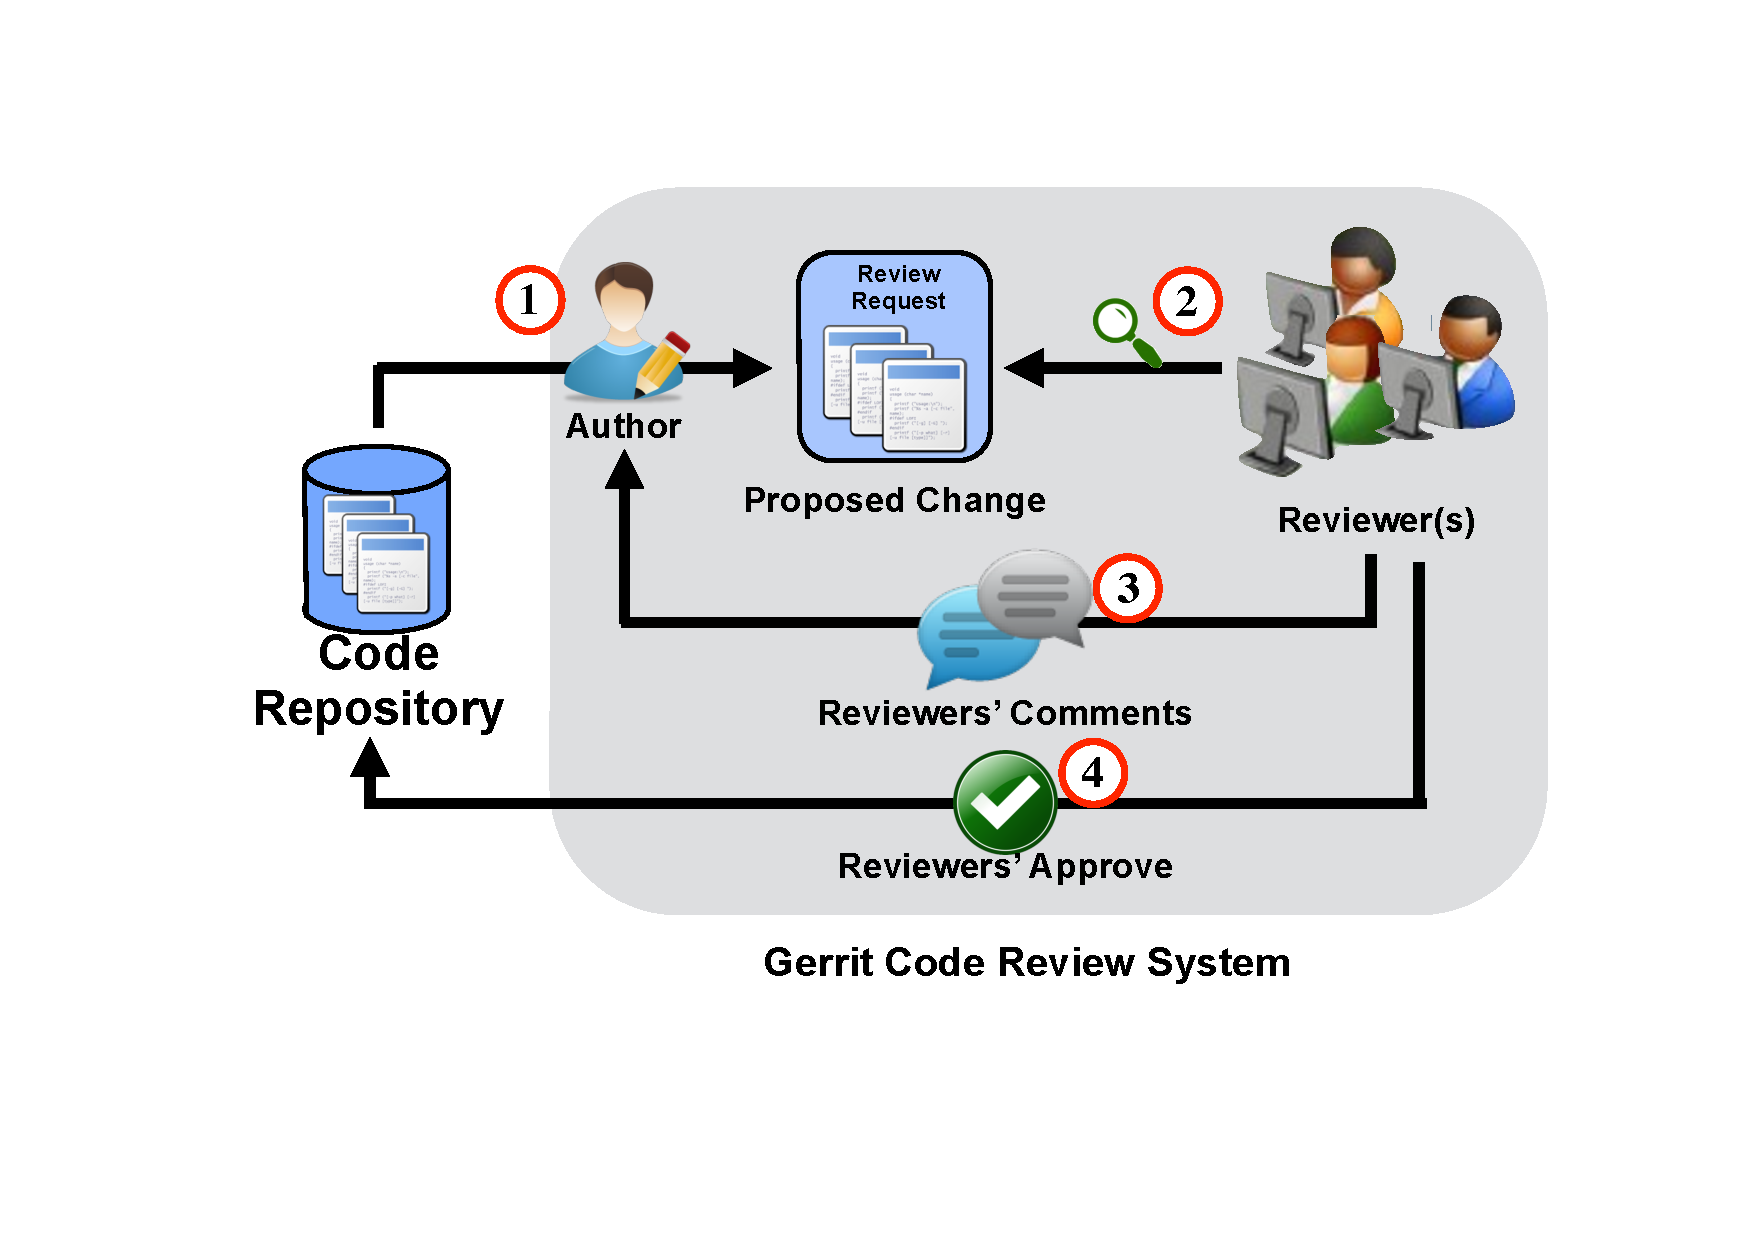
\includegraphics[scale=0.35, trim= 100 110 50 80, clip=true]{review_process}
\caption{An simplified version of MCR Process based on Gerrit system}
\label{fig:process}
\end{figure}
% !TEX root = ../paper.tex

%\section{Background}
%In this section, we describe MCR process based on Gerrit system. Then, we describe the background behind our approach composed of text mining techniques using VSM and euclidian distance and prediction evaluation techniques. 
%\dan{this section seems to only cover MCR. We could have this be a Background section with this and the other subsequent sections moved to sub-sections}

\section{Modern Code Review Process}

An overview of MCR process based on the Gerrit code review system is shown in Fig. \ref{fig:process}.
The grey area shows the review process of the system which is composed of four main steps:
(1) An author creates a patch and submits a set of new or modified files as a review request to the Gerrit system.
(2) Reviewers examine the proposed code changes for defects or concerns.
(3) Reviewers provide comments to the author.
The author creates a revised proposed change according to the comments and re-submits for review.
Reviewers then examine the revised proposed change.
If the revision is not approved, reviewers provide comments to fix and the process continues until
(4) reviewers can determine that a proposed change can be merged into the project (approved change) or should not be merged (rejected).


According to this process, reviewers' comments are the most important factor in determining software quality.
In particular, McIntosh et. al. \cite{Mcintosh} found that components which were reviewed without discussion (i.e. no comments) are likely to contain bugs.
However, it has not been shown that components with comments are less likely to contain bugs. Tools supporting MCR such as Gerrit allow reviewers to freely write messages to authors (and other reviewers), and frequently, these comments are superficial or do not clearly identify defects or relevant issues for the proposed change and are thus of questionable usefulness and consequently may have little impact on quality.
% (e.g. coding styles, documentation, process workflow, etc.)
For example, a comment may be related to something outside the scope of the proposed change, perhaps author or reviewer personal issues or inter-personal communication e.g. ``Keep up the good work everyone!".
Microsoft developers reported that the reviewers often only focus on minor logic errors rather than discussing deeper design issues \cite{Bacchelli2013a}.
Our observations of the Qt project also corroborate this finding.
We found that many examples of comments that are superficial and unhelpful to the proposed changes.
For example, the superficial and unconfident comment shown in Fig. \ref{fig:example}(a) is certainly within the scope of the proposed change, yet provides little useful information.
While the comment in Fig. \ref{fig:example}(b) about using the version control system (in this case Git) is clearly out of scope, and not directly useful for the proposed change. 

Ultimately our aim is to understand the impact of useful and useless comments on code quality. Specifically, what degree of useful comments are needed to effect positive impact on quality. Study of this necessitates ascertaining, with high confidence, the usefulness of a large number of comments. This  had proven difficult to accomplish manually, so here we investigate the pragmatics of using semantic similarity to assist with this task.


\begin{figure}[!t]
\centering
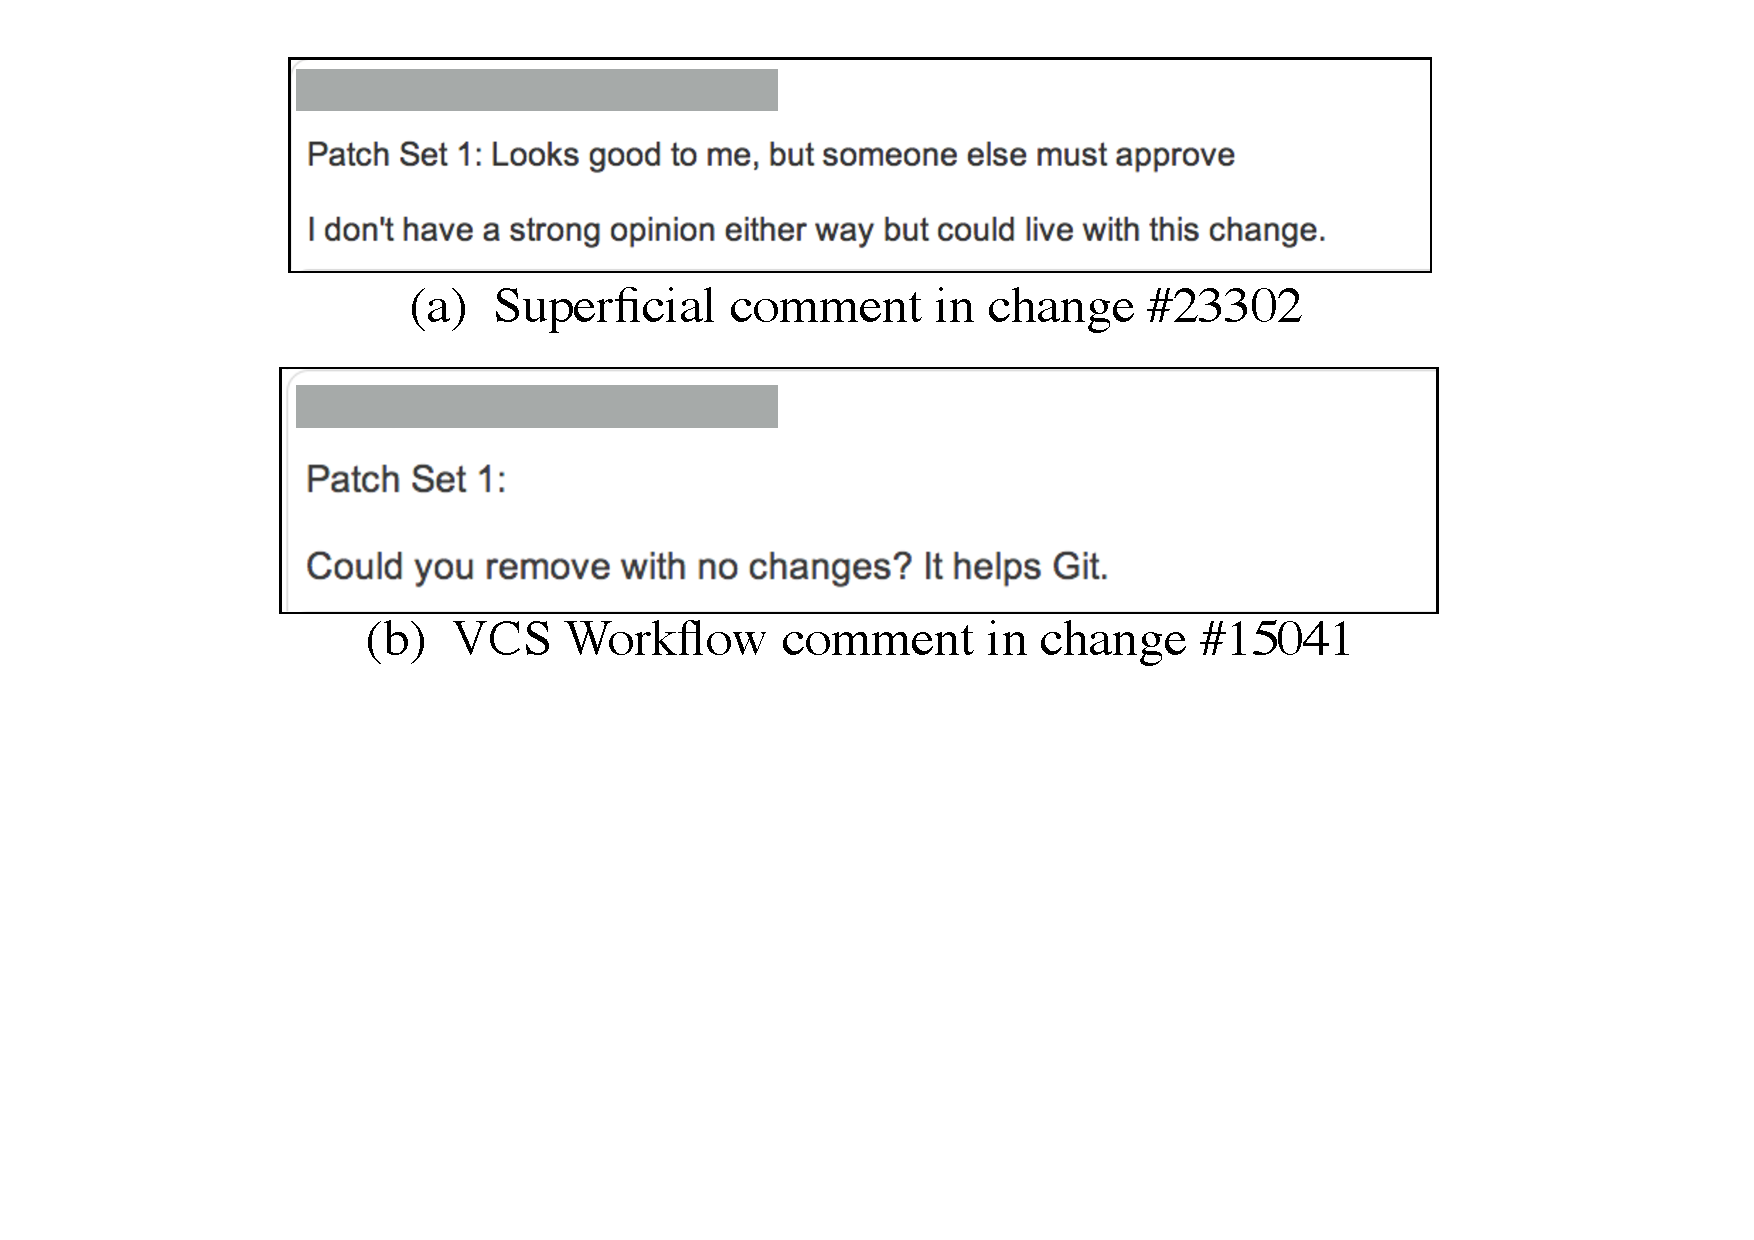
\includegraphics[scale=0.4, trim= 100 250 0 0, clip=true]{comment_examples}
\caption{Examples of comment in code reviews of Qt project.}
\label{fig:example}
\end{figure}

% !TEX root = ../paper.tex

\section{Semantic Similarity Classification of Comment Usefulness}

\textbf{Definition:} We define a \emph{useful} comment as one that contributes to improving the proposed change, and a \emph{useless}\footnote{Although we call these comments \emph{useless} in our study, it might actually be useful---or sometimes even required---in some other contexts, such as to facilitate communication or to enforce guidelines.} comment as one that does not.

Our goal is to improve the efficiency and confidence in determining the usefulness of review comments.
Usefulness is not dichotomous and hence we must accept a third qualification, \emph{unclear}, to allow for the case where a comment does not directly make a positive contribution but is not clearly out of scope or tangential.
Therefore, our approach is largely based on relevance the comment has to the proposed change (as documented within a MCR system).
A primary factor in relevance is similarly, and so it is natural for us to consider classification using \emph{similarity conditions}\cite{Davies2012}. 
%\dan{can we find a reference for relevance and similarly?}
We assume that the more similar a comment is to the proposed change, the more relevant it is and hence more likely useful.
Conversely, the more dissimilar\footnote{This can be arbitrarily large, thus not simply the opposite of similarity}, the less relevant, and hence less useful.

\subsection{Approach}
Given the subjective nature of usefulness, precise classification conditions probably do not exist and so we resort to conditions that indicate a meaningful \emph{likelihood} of classification.
That is, for some degree of similarity a comment is most likely useful, and for some degree of dissimilarity it is most likely useless.
The key is to determine these degrees in a practical and effective manner.

Fig. \ref{fig:overview} shows an overview of our proposed classification approach.
Usefulness of a comment is determined by computing its semantic similarity with the commit message of its proposed change and observing if it satisfies \emph{usefulness classification likelihood conditions}.
The conditions are simply threshold values of similarity and dissimilarity empirically determined to optimize a desired likelihood objectives.


\begin{figure}[!t]
\centering
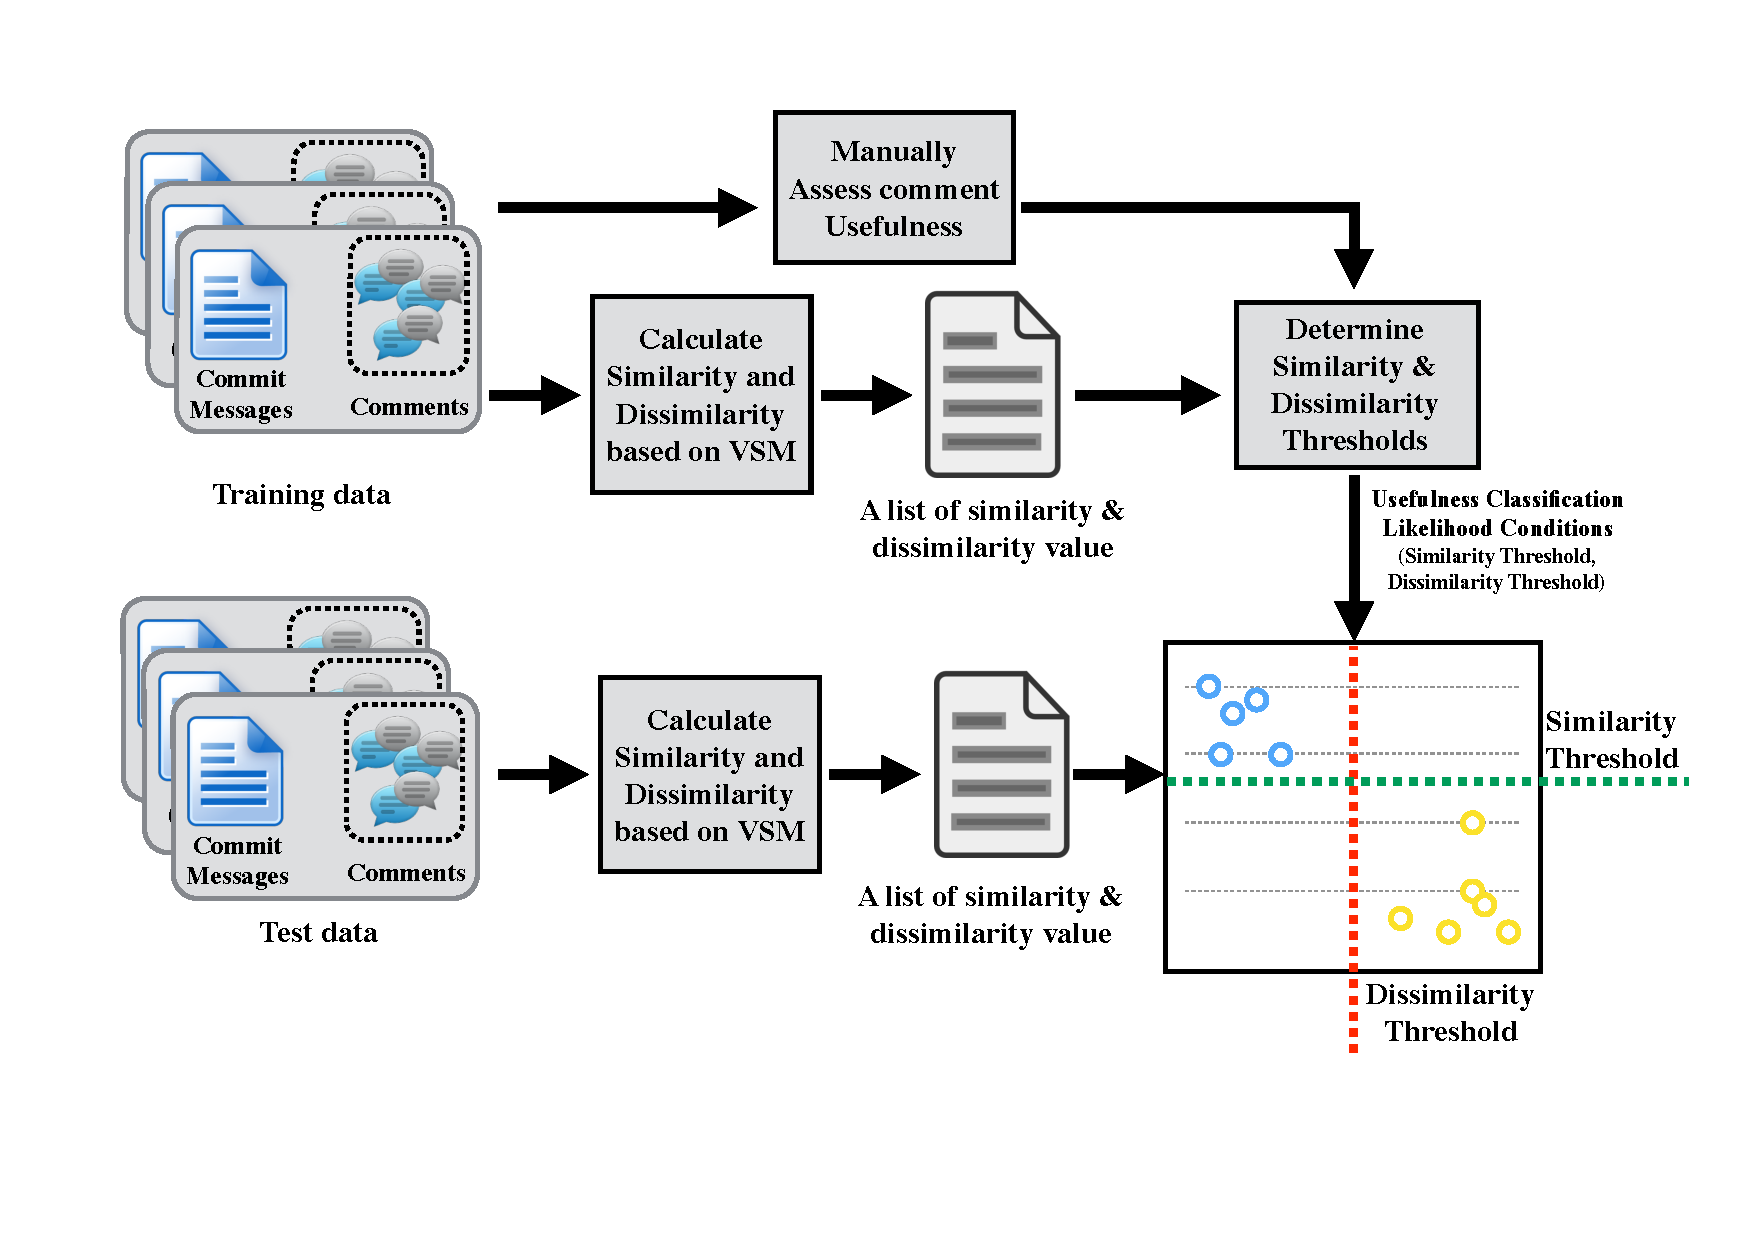
\includegraphics[scale=0.34, trim = 50 90 0 30, clip=true]{overview2}
\caption{An overview of classification of comment usefulness using semantic similarity}
\label{fig:overview}
\end{figure}

% again, I can't see Fig. \ref{fig:overview}(a)
% Thai sez: Cosine distance IS NOT cosine similarity. Cosine distance is defined as 1 - cosine similarity, and is not a proper distance metric, lacking triangle equality and stuff [Wikipedia].
We calculate semantic similarity using the Vector Space Model (VSM) with the cosine similarity measure, which is a well-known technique for retrieving relevant documents written in unstructured natural language; and the Euclidian distance, which is a well-established measure of dissimilarity and applies analogously.
%For our case example training dataset, we manually identified 320 randomly-selected pairs of comments and corresponding commit messages in Fig. \ref{fig:overview}(b). \thai{The %overview figure does not have (a) and (b)...}
%\dan{what was the actual effort (in person-hours) to create the training data?}

Our training data is a small set of randomly-selected pairs of comments and the corresponding commit messages.
These comments are manually assessed for usefulness.
%Each comment is assessed by three different people independently.
%For each \texttt{YES} vote, a single point is given to that comment.
%This means that a comment will receive a score of 0, 1, 2, or 3.
For statistical purposes, at least 30 useful and 30 useless comments must be collected.
The similarity and dissimilarity metrics are then computed for the data set.
These are used to estimate the similarity and dissimilarity thresholds $S_T$ and $D_T$ that best discriminate useful comments and $S'_T$ and $D'_T$ for useless comments. 
%Other likelihood functions could be used depending on precision, recall, or risk goals.
We find these thresholds by selecting $s_t,d_t$ values that maximize the F-measure,
which is a performance measure for a binary classification that compromises trade-offs in accuracy of classification (precision) and coverage of classification (recall).
In this study, we used the F$_1$-measure, which equally prioritize precision and recall.
Different weighting can be used by different F$_\beta$ measures depending on an application.


\subsection{Usefulness Classification Conditions} 
Using those thresholds, we can classify the usefulness of comments for the rest of comments (as test data) in review history according to the classification model as follows: given a comment $c$ and a corresponding commit message $m$,
\begin{itemize}
\item \textbf{useful}: $\Theta(c,m,S_T,D_T) = \True$ iff $\Sim(m,c) \geq S_T$ and $\Dist(m,c) \leq D_T$.
\item \textbf{useless}: $\Omega(c,m,S'_T,D'_T) = \True$ iff $\Sim(m,c) \leq  S'_T$ and $\Dist(m,c) \geq D'_T$.
\item \textbf{undetermined}: neither or both of the above conditions are $\True$.
% We also refer to them as \emph{neither} and \emph{overlap}.
\end{itemize}

The functions $\Sim(m,c)$ and $\Dist(m,c)$ are the similarity and dissimilarity measures relative to the proposed change commit message $m$ for the text of comment $c$ using cosine similarity and euclidian distance, respectively.
Two metrics are used because they are independently generated and thus provides better discrimination for classification.
We also found experimentally that using two metrics has higher performance than just one. 

% The details of our approach are elaborated in the following subsections.

%\dan{**** ALERT **** this entire subsection is not needed! Everything in it is well-known and can simply be referenced. I suggest removing it if we need the space.  I have not edited this section .... }
%\subsection{Similarity and Dissimilarity Calculation based on VSM}
%%Vector Space Model (VSM) is well-known technique for information retrieval where documents written in unstructured natural language. In Software Engineering, VSM has been widely use to find relationship among documents in software issue tracking system\cite{Davies2012}.
%For each review, we compute similarity and dissimilarity of every comments comparing with the commit message which is described the purpose of the change.
%To do so, we use VSM which is a model for representing text documents as vectors.
%For a set of commit messages and comments ($D$), each document, $d$ (commit message or comment) is represented as $\overrightarrow{V_d} = <w_{1,d},w_{2,d},w_{3,d},...w_{n,d}>$, where $n$ is the total number of unique terms occur in $D$.
%The $w_{t,d}$ value is tf-idf weighting of term $t$ calculated from term occurrence frequency using Equation \ref{eq:tf-idf} where $\operatorname{tf}_{t,d}$ is frequency of term $t$ occurs in document $d$; and $|\{d' \in D | t \in d'\}|$ is the number of other documents $d'$ that also contain term $t$.  
%
%\begin{equation}
%w_{t,d} = \operatorname{tf}_{t,d} \times \log\frac{|D|}{|\{d' \in D \:|\: t \in d'\}|}
%\label{eq:tf-idf}
%\end{equation}
%
%After transforming commit message and comments to vectors, we calculate similarity using Cosine similarity and Euclidian distance. 
%
%
%\noindent\textbf{Cosine similarity} measures similarity between two vectors using inner product. Given a vector commit message $\overrightarrow{V_m}$ and the vector of its comments $\overrightarrow{V_m}$, we can calculate Cosine similarity using Equation \ref{eq:cosine}. The similarity value is ranging $[0,1]$ where 0 means there is no similarity and 1 means two vectors are textually similar.  
%
%\begin{equation}
%\Sim(c) = \cos\theta(\overrightarrow{V_m},\overrightarrow{V_c}) = \frac{\sum_{i=1}^{|D|} w_{i,m} \times w_{i,c}}{\sqrt{\sum_{i=1}^{|D|} w^2_{i,m} \times \sum_{i=1}^{|D|} w^2_{i,c}}}
%\label{eq:cosine}
%\end{equation}
%
%\noindent\textbf{Euclidian distance} measures ordinary distance between each element of two vectors using Equation \ref{eq:euclid}. We can use this distance as an dissimilarity. Given a vector commit message $\overrightarrow{V_m}$ and the vector of its comments $\overrightarrow{V_m}$, we can calculate Euclidian distance using Equation \ref{eq:cosine}. The distance value is ranging $[0,\infty)$ where 0 means these vectors are the same vectors while a more distance means these vectors are less similar.
%
%\begin{equation}
%\Dist(m,c) = \|\overrightarrow{V_m} - \overrightarrow{V_c}\| = \sqrt{\sum_{i=1}^{|D|}(w_{i,m} - w_{i,c})^2}
%\label{eq:euclid}
%\end{equation}
%
%\subsection{Estimating Similarity and Dissimilarity Thresholds}
%Suppose we use $\Theta(c,S_T=s_t,D_T=d_t)$ to classify useful comments and we have the following values:
%
%$\mathrm{TP}_{s_t,d_t}$ is the number of comments that our model classified as \textit{useful} and are \textit{actually useful} i.e. true-positives; 
%
%$\mathrm{FP}_{s_t,d_t}$ is the number of comments that our model classified as \textit{useful} but are \textit{actually useless} i.e. false positives;
%
%$\mathrm{FN}_{\theta_s,\theta_d}$ is the number of comments that our model classifies as \textit{useless} but are \textit{actually useful}. 
% 
%We can now define the following classification  performance measures: 
%\begin{equation}
%\begin{split}
%\mathrm{F\text{-}measure}_{s_t,d_t} &= 2 \times \frac{\mathrm{precision}_{s_t,d_t} \times \mathrm{recall}_{s_t,d_t}}{\mathrm{precision}_{s_t,d_t} + \mathrm{recall}_{s_t,d_t}}
%\\
%\mathrm{precision}_{s_t,d_t}  &= \frac{\mathrm{TP}_{s_t,d_t}}{\mathrm{TP}_{s_t,d_t}+\mathrm{FP}_{s_t,d_t}}
%\\
%\mathrm{recall}_{s_t,d_t}  &= \frac{\mathrm{TP}_{s_t,d_t}}{\mathrm{TP}_{s_t,d_t}+\mathrm{FN}_{s_t,d_t}}
%\end{split}
%\label{eq:fmeasure}
%\end{equation}

% Our proposed approach is empirically driven and automatically adjusts to the quality the data.
While our proposed approach is straightforward, empirically driven, and automatically adjusts to the quality of the data, it has a few drawbacks.
We have to accept that some comments cannot be reliably or confidently classified.
We denote these as \emph{undetermined} to differentiate them from comments whose usefulness is \emph{unclear} (i.e. cannot be assessed subjectively).
Secondly, owing to the subjective assessment of usefulness, this representation fundamentally implies supervised classification requiring nontrivial training data to define representative classification sets.


% empirically driven and automatically adapts to the quality the data


% Thai sez: We did not mention the F-measure for \Theta, thus suddenly referring to \Omega does not make much sense...
% The F-measure for $\Omega(c,S_T=s_t,D_T=d_t)$ is computed analogously where we change instances of useful to useless and vice-versa in the definitions. The correctness of classification is determined from the useful/useless defined dataset. 


%Using this method, we iteratively measure an accuracy for values of $s_t$ and $s'_t$ ranging $[0,1]$; and values of $d_t$ and $d'_t$ ranging $[0,\infty)$. 

%\begin{equation}
%\mathrm{F\text{-}measure}_{S_T,D_T} = \frac{2\mathrm{TP}_{S_T,D_T}}{2\mathrm{TP}_{S_T,D_T}+\mathrm{FP}_{S_T,D_T}+\mathrm{FN}_{S_T,D_T}}
%\label{eq:precision}
%\end{equation}

%where $\mathrm{TP}_{S_T,D_T}= |\{ c \in C |  \text{\textbf{useful}}(c,S_T,D_T) = \mathrm{TRUE} \}\cap \{c \in C| \mathrm{vote}(c) = 2\}|$,  $\mathrm{FP}_{S_T,D_T} = |\{ c \in C | \text{\textbf{useful}}(c,S_T,D_T) = \mathrm{FALSE} \}\cap \{\mathrm{vote}(c) = 2\} $, $\mathrm{FN}_{S_T,D_T} = |\{ c | c \in C, \text{\textbf{useful}}(c,S_T,D_T) = \mathrm{TRUE} \}\cap \{\mathrm{vote}(c) < 2\} $
%According to this, we can formalize as follows:

%\begin{equation}
%(S_T,D_T) = \max(\{\mathrm{F\text{-}measure} \text{ of \textbf{useful}}(c,s_T,d_T) | s_T\in[0,1] \text{ and } d_T\in [0,\infty) \})
%\end{equation}

% !TEX root = ../paper.tex

\section{Case Study}


Our case study used the Qt project review history from the Gerrit code review tool provided by Hamasaki et. al. \cite{Hamasaki2013}. Qt project is a large open source project composed of numerous small subsystems. We selected the most active subproject \texttt{qtbase} project. From this project, we used the review history from \TODO{Month-Year} to \TODO{Month-Year} which has \TODO{XX} reviews and \TODO{XX} comments.


% where we got the data
%We used the review data sets of the Qt project collected by Hamasaki et al\cite{Hamasaki2013}.
%Only reviews in the master branch of \texttt{qtbase} project are considered,
%as it is the most active branch.

% quick structure
%\pick{This already explain in background :D}
%Each change includes a \emph{commit message} which describes what is changed.
%After a change is submitted to Gerrit, reviewers can give scores to it.
%The scores will determine whether the change will be accepted or not.
%Reviewers can also add comments to the change, which may optionally be added to a specific line of code inside a changed file.
%Majority of the comments are automatically generated by Gerrit and do not contain any user-written text.

% overview
%In our classification method,
%all commit messages and comments that are human-written are converted into vectors using tf--idf algorithm.
%Few comments are sampled and then classified manually for use in training and validation.
%A model is created from these training data, from which useful comments can automatically be identified.
%This process is illustrated in Fig.\ref{fig:overview}.
%



\subsection{Data Preparation}
We used commit messages and comments in the dataset. Before classifying the usefulness of comments, we first processed the commit message and comments as follows: 

\subsubsection{Automatically generated messages removal}
In Gerrit, the comments are composed of comment messages from reviewers and automated messages. These automatic messages are generated by Gerrit and the integration system to record activities. For example, \textit{'Upload patch set 1.'}, \textit{'Change has been successfully cherry-picked to the staging branch as ...'}. Since these messages are generally recored keeping, they are not substantially relevant to the proposed changes and do not directly impact software quality\cite{Mcintosh} and hence are useless by our definition. In practice they are not considered in code review. They are easily determined as useless by our method and would artificially improve our classification performance. We identified these automatic messages using regular expressions and selecting frequently appeared patterns of messages.  


%The commit messages and all comment texts are converted into vectors as part of the preparation step.
%Fig. \ref{fig:preprocess} illustrates the overview of this step.
%We wrote scripts in Ruby language to perform these tasks.

%\begin{figure}[h]
%\centering
%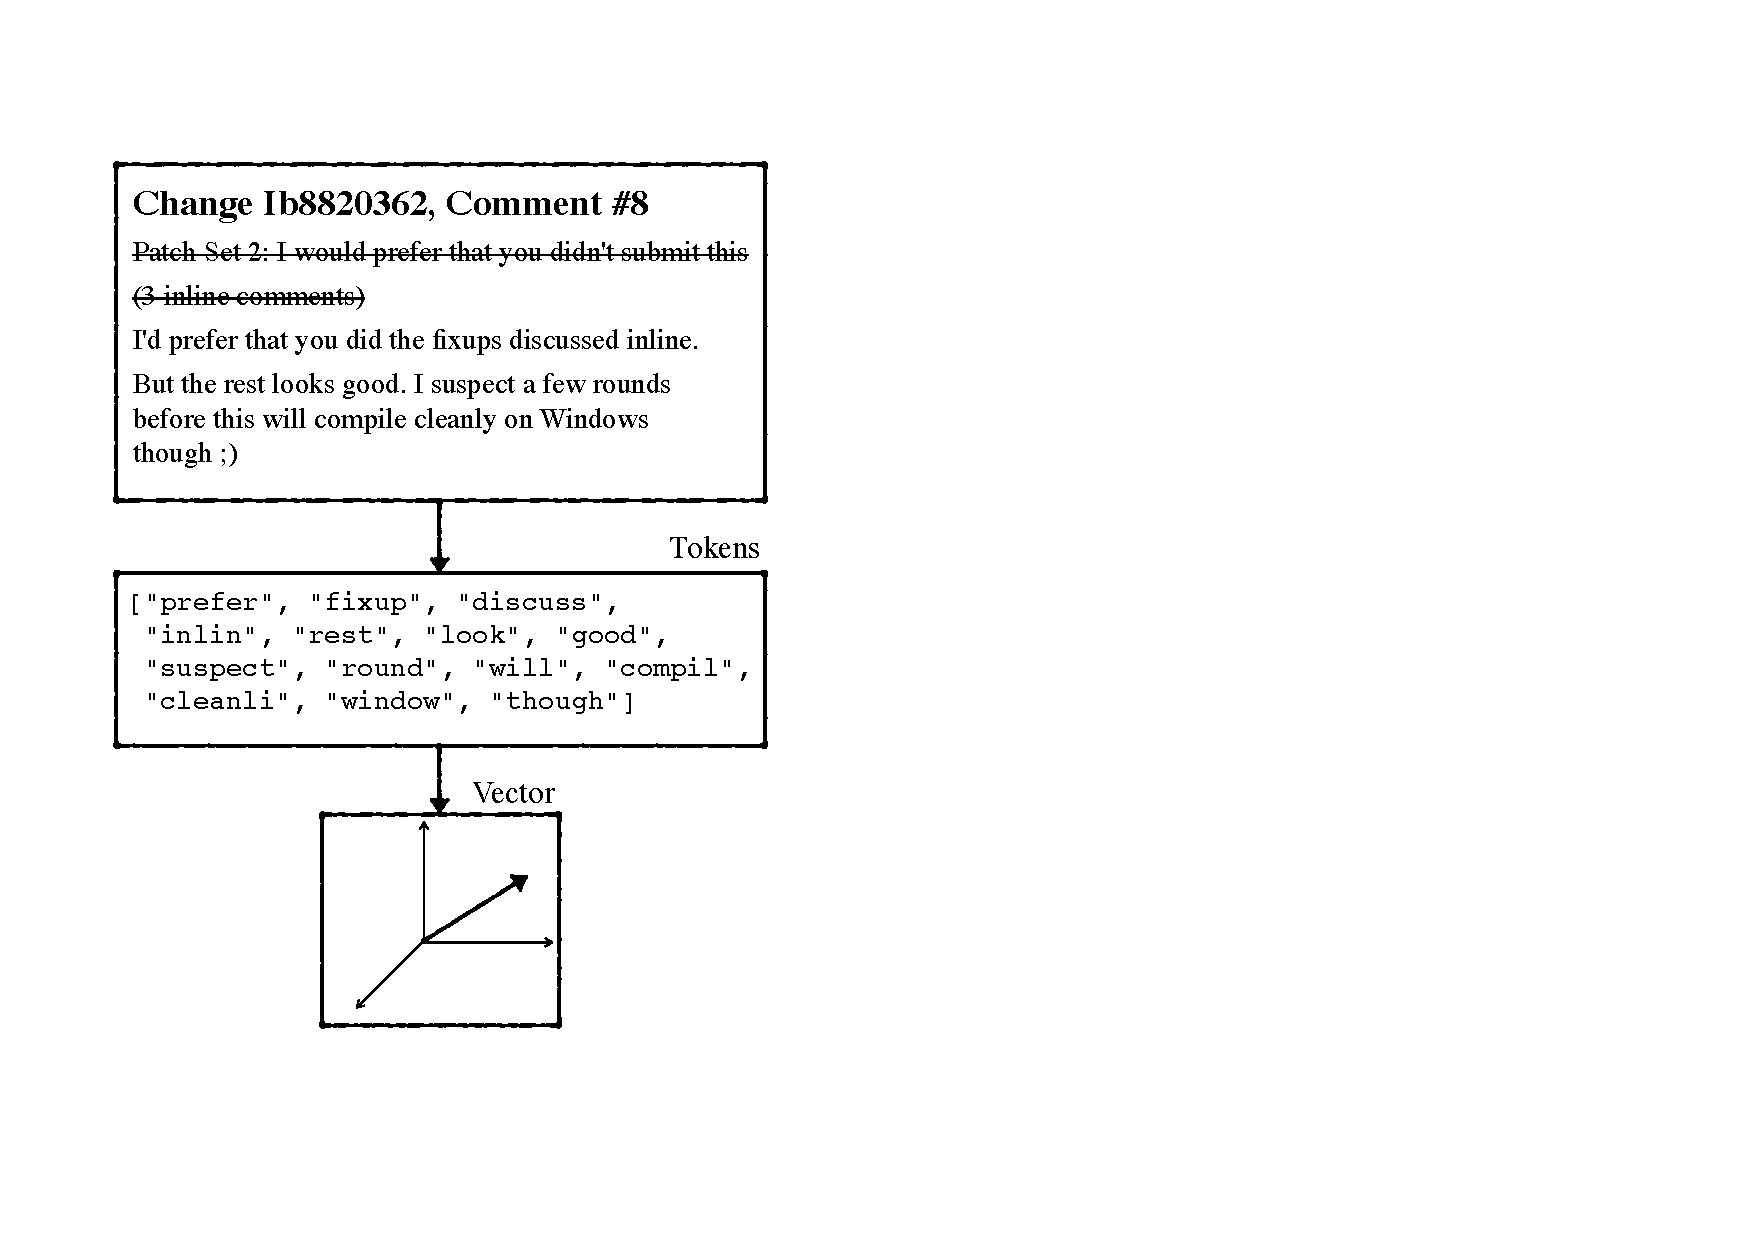
\includegraphics[width=3in]{preprocess}
%\caption{The data preparation process.
%Automatically generated texts are removed, remaining text is tokenized, stop words are removed, remaining tokens are stemmed,
%and are converted into a vector.}
%\label{fig:preprocess}
%\end{figure}



%\subsubsection{Removal of automatically generated text}
%
%First, all comments by the Gerrit system, \emph{Qt Sanity Bot}, and \emph{Qt Continuous Integration System} are skipped.
%
%% conversion into vector, wow
%Next, we looked for common patterns that appeared in the comments, because it is very likely that they are automatically generated.
%This is accomplished by splitting texts into lines, and for each line, searching for words that can be found in the English wordlist\footnote{The wordlist found in \texttt{/usr/share/dict/words} from Ubuntu Linux distribution is used.}.
%This effectively removed the ID numbers and other non-generic terms.
%
%Next, the lines that appears most frequently are identified.
%From these lines, we then constructed the regular expression patterns,
%and finally, these patterns are used to filter out automatically generated text from our data.



\subsubsection{Data Preprocessing}
 As is customary for VSM processing we extracted semantic words from commit messages and comment messages before converting to vector. For each message, we removed all punctuation signs, digits, and common words (e.g. a, an, the) using Google stop word list\footnote{Available at \url{http://meta.wikimedia.org/wiki/Stop_word_list/google_stop_word_list#English}}. We then used Porter stemming algorithm to remove the commoner morphological and inflexional endings from words in English.
 


%After the automatically generated messages are removed, we extracted the words in each document into a list of tokens by searching for alphanumeric characters including apostrophes.
%Stop words from the Google stop word list\footnote{Available at \url{http://meta.wikimedia.org/wiki/Stop_word_list/google_stop_word_list#English}} are then removed.
%The stemming is performed on remaining tokens using Porter stemming algorithm.
%The remaining words are then combined to form a corpus of all used words.



%\subsubsection{Conversion into vector}
%
%Finally, the tf--idf algorithm is used to convert each document into a vector.

\subsubsection{Ground-Truth Data Preparation}
To prepare ground-truth data, a team of three experienced developers independently read comments and manually assessed them useful or useless. The assessors were asked to answer for each comment the question ``Does this comment technically contribute to its proposed change?''. Then, the assessors cast their vote as \texttt{YES} if the comment is likely to useful and \texttt{No} if the comment is likely to useless.  Comments with three \texttt{YES} votes are classified as \textbf{useful} comments and comments with three \texttt{NO} votes are \textbf{useless}. Comments lacking unanimity (i.e. one or two \texttt{YES} votes are deemed \textbf{unclear} and without confident usefulness. 

\subsection{Research Questions}
To validate our approach, we addressed the following research questions:

\noindent \textbf{RQ1: Is semantic similarity a good indicator of MCR comment usefulness?}\\
\indent To answer this question, we randomly sampled 320 comments from our data set and manually identified usefulness as described in previous subsection. Then, we used these comments for both the training and test data set for our approach to determine its effectiveness. We also determined the robustness of our approach using cross validation. We randomly selected 90\% of 320 comments for training set and 10\% for test set.
The effectiveness was measured using precision, recall and F-measure as described in Equation \ref{eq:fmeasure}. We repeated this validation for 300 times and find average of accuracy.

\dan{What what the effort in person-hours for this?}

Since our models do not include unclear type of comments, we defined them as negative condition i.e useless comments in case of useful classification (when using $\Theta(c,S_T,D_T)$ model) and useful comments in case of useless classification (when using $\Omega(c,S'_T,D'_T)$ model).


%We sampled 320 comments from the data set.
%These samples are then classified as either useful (that is, technically contributing to the software) or not useful.
%This task is carried out by three people who worked independently.
%
%Each comment is then scored based on the number of positive answers.
%For example, a comment with a score of 3 means that all three people said that it is useful,
%while a comment with a score of 0 means that none of us marked it as useful.


\noindent \textbf{RQ2: Do code reviewers intensively discuss on the proposed changes?}\\
\indent To answer this question, we estimated similarity and dissimilarity thresholds using comments from RQ1 for training set. We then used these thresholds to classify the rest of comments. A statical analysis was performed to understand the impact of useful discussion to software quality.

\noindent \textbf{RQ3: Does this approach practical and cost-effective for large-scale projects?}\\
\indent




%\subsection{Training Data}



%The score of a comment can be defined as:

%\begin{align*}
%Score_i & = \sum_{\text{reviewer } r} Review(r, i). \\
%Review(r, i) & = \begin{cases}
%	1 & \text{if } r \text{ says that the comment } i \text{ is useful,} \\
%	0 & \text{otherwise.}
%\end{cases}
%\end{align*}



%\pick{I re-wrote of these, hope I don't miss something ;)}
%\subsection{Model Generation and Validation}
%
%% the metrics
%For each comment, we computed similarity and dissimilarity metrics
%between the comment text and the corresponding commit message.
%We chose cosine similarity and euclidean distance as the metrics to use in model generation.
%
%\begin{figure}[h]
%\centering
%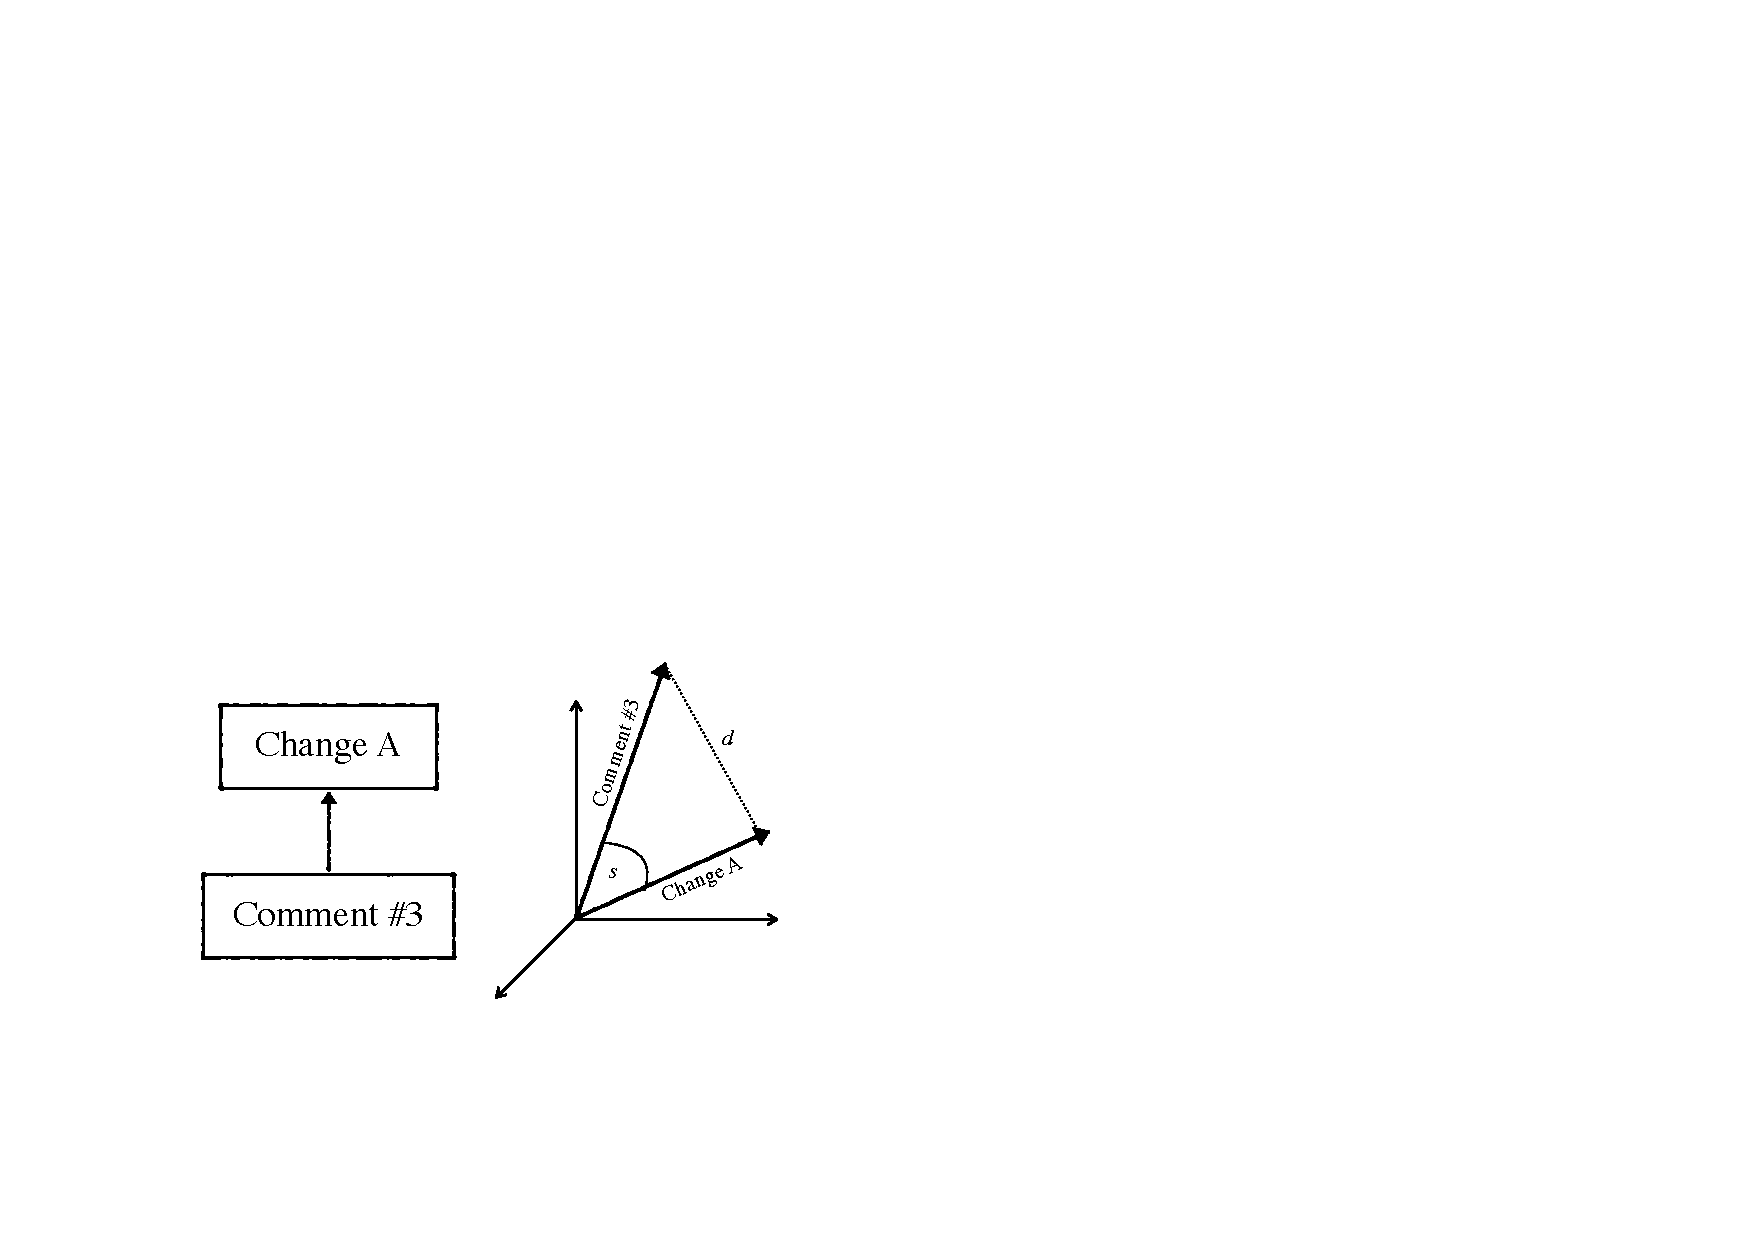
\includegraphics[width=3in]{vector}
%\caption{The similarity and distance metric that is being used.}
%\label{fig:vector}
%\end{figure}
%
%% assumptions in categorization
%The model is based on two assumptions: that useful comments will have a $similarity \geq A \text{ and } distance \leq B$,
%and that comments that are not useful will have a $ similarity \leq C \text{ and } distance \geq D$,
%where $A$, $B$, $C$, and $D$ are some constant.\footnote{We also tried using the `or' operator, and found that using `and' produces better result.}
%
%% finding parameters
%To find these parameters, a brute-force approach is used.
%This is possible because the set of $similarity$ and $distance$ values are discrete.
%Each possible value of $A$, $B$, $C$, and $D$ are evaluated to find the constant that returns the maximum F$_1$ score.
%
%% validation
%To validate our model, we randomly split the data into 10 parts.
%9 parts are used for training, and 1 part for validation.
%This process is repeated 300 times. % while I sleep
%The values of precision, recall, F$_1$ score, and accuracy are recorded and then averaged
%to give the overall performance of our model.


% !TEX root = ../paper.tex

\section{Case Study}

Our case study used the Qt project review history from the Gerrit code review tool provided by Hamasaki et. al. \cite{Hamasaki2013}. Qt project is a large open source project composed of numerous small subsystems. We selected the most active subproject, which is called \texttt{qtbase}.
From this subproject, we used the review history from May 2011 to June 2012, which contains 6,605 changes and 72,484 comments.


\subsection{Data Preparation}
We used the commit messages and comments in the dataset.
Before classifying the usefulness of comments, we first processed the commit message and comments as follows: 

\subsubsection{Removal of automatically generated messages} To consider only reviewers discussion, we ignored all messages that automatically generated.
%In Gerrit, the comment history is composed of human-written comments from reviewers and automatically generated messages.
These automatic messages are generated by Gerrit, continuous integration system, and the sanity bot\footnote{It is a bot that automatically checks new proposed changes for trivial sanity issues, such as line endings, copyright notices, and commit messages} to record activities. \textit{`Upload patch set 1.'}, \textit{`Change has been successfully cherry-picked to the staging branch as ...'}, and \textit{`Sanity review passed'} are some examples. In practice, they are not considered in code review  and are not substantially relevant to the proposed changes and do not directly impact software quality\cite{Mcintosh}. 

To do so, we first ignore all comments written by bots (i.e. \emph{Qt Continuous Integration System} and \emph{Qt Sanity Bot}). Second, we removed message including reviewers comments by finding common patterns frequently occurred using regular expression. This would leave us only human-written comments that will be used in further preprocessing.

%, . and hence are useless by our definition.
%%They are easily determined as useless by our method and would artificially improve our classification performance.
%These messages are identified by looking for the most common lines of text using regular expression.
%%Regular expression patterns are then constructed to match and remove these messages.
%Occurrences of these patterns are then removed from our dataset prior to further preprocessing.
%
%Automatic messages are also often inserted as part of review comments.
%They too are removed from our dataset, leaving us with only human-written part.
%We also completely ignored comments whose author is \emph{Qt Continuous Integration System} and \emph{Qt Sanity Bot}.

\subsubsection{Data preprocessing}
As is customary for VSM processing, we extracted semantic words from commit messages and comment messages before converting to vector.
For each message, we removed all punctuation signs (except apostrophe) and other non alphanumeric characters. We also removed common words (e.g. a, an, the) using Google stop word list\footnote{Available at \url{http://meta.wikimedia.org/wiki/Stop_word_list/google_stop_word_list#English}}. We then used Porter stemming algorithm to remove the commoner morphological and inflexional endings from words in English.

Table \ref{tb:datastatistic} summarizes data set we used for this study after preparation. 

\begin{table}[!h]
\caption{A summary data sets and some statistics.}
\centering
\small
\begin{tabular}{ccc}
\hline
& Total Number & Percentage \\ \hline \hline
Commit Messages & 6,605 &  -  \\ \hline
All Comments & 72,484& - \\ \hline
Reviewers Comments & 10,583 & 15\% \\ \hline
Automated Comments & 61,814 & 85\% \\ \hline 

\end{tabular}
\label{tb:datastatistic}
\end{table}

\subsection{Manual Comment Usefulness Assessment}
In this case study, three participants (the first two authors and one student) independently classified comments by giving a question, ``does this comment technically contribute to its change or not?''
Then, the participants gave a vote for \texttt{YES} if the comment is likely to be useful and \texttt{NO} otherwise.
From the voting scores, we regarded that the comments with three \texttt{YES} votes are \emph{useful} comments and the comments with no \texttt{YES} votes (i.e. three \texttt{NO} votes) are \emph{useless} comments. For the comments with one and two \texttt{YES} votes, we defined them as unclear comments.

\subsection{Research Questions}
% We addressed two research questions: \textbf{RQ1:} Is semantic similarity a good indicator of MCR comment usefulness? and \textbf{RQ2:} Is semantic similarity classification cost-efficient, assurable, and scalable?.
% \pick{Do we need motivation for these RQs?}
% Thai sez: these recitation of research questions are very redundant...
%           for the motivation, I think it should have been discussed at the introduction.

%\pick{I realize that your figure is better for the presentation :)}
%\begin{figure}[h]
%\centering
%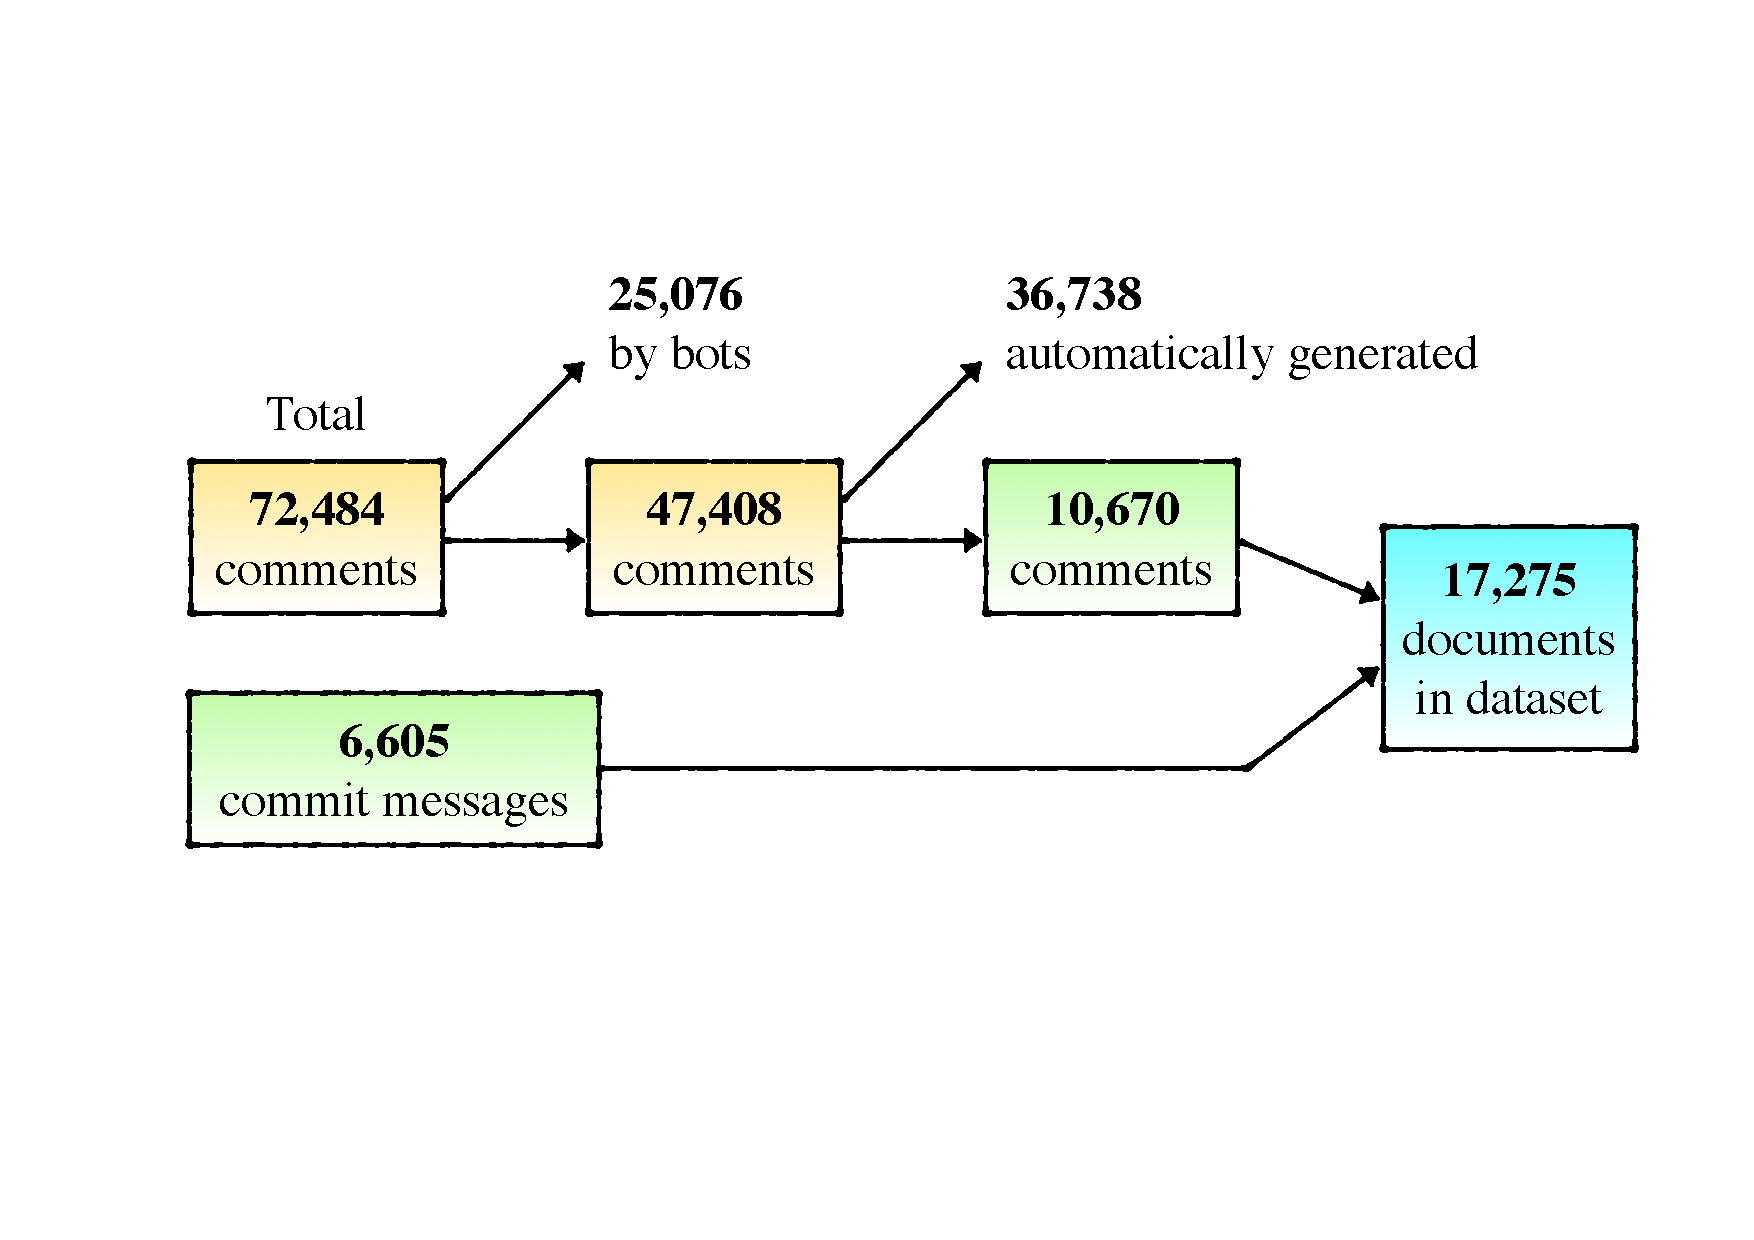
\includegraphics[width=3.2in]{filter}
%\caption{The filtering process.}
%\label{fig:filter}
%\end{figure}
%\subsection{Data Preparation}
%\subsubsection{Data extraction}
%
%6,605 changes and 72,484 comments have been extracted from the raw dataset.
%35\% of the comments are by the system or one of the bots, and are thus discarded.
%
%\subsubsection{Common pattern removal}
%
%By looking for most frequent lines, common patterns were found, such as \emph{`Uploaded patch set 2.'} and \emph{`Change has been successfully cherry-picked to the staging branch as \dots'}.
%
%Removing occurrences of these patterns leaves 77\% of the remaining comments empty.
%This probably means these comments solely contain automatically-generated text, and are thus discarded.
%This leaves us with 10,670 comments and 6,605 commit messages; a total of 17,275 documents.
%
%\subsubsection{Tokenizing}
%
%After the tokenization step, 393,238 tokens are generated in total. They are composed of 20,025 different words.
%This means that each document will be converted into a vector of 20,025 dimensions, each dimension representing a single word.


\begin{ResearchQuestions}
\item[RQ1:] Is semantic similarity a good indicator of MCR comment usefulness?
\end{ResearchQuestions}

\begin{figure}[!t]
\centering
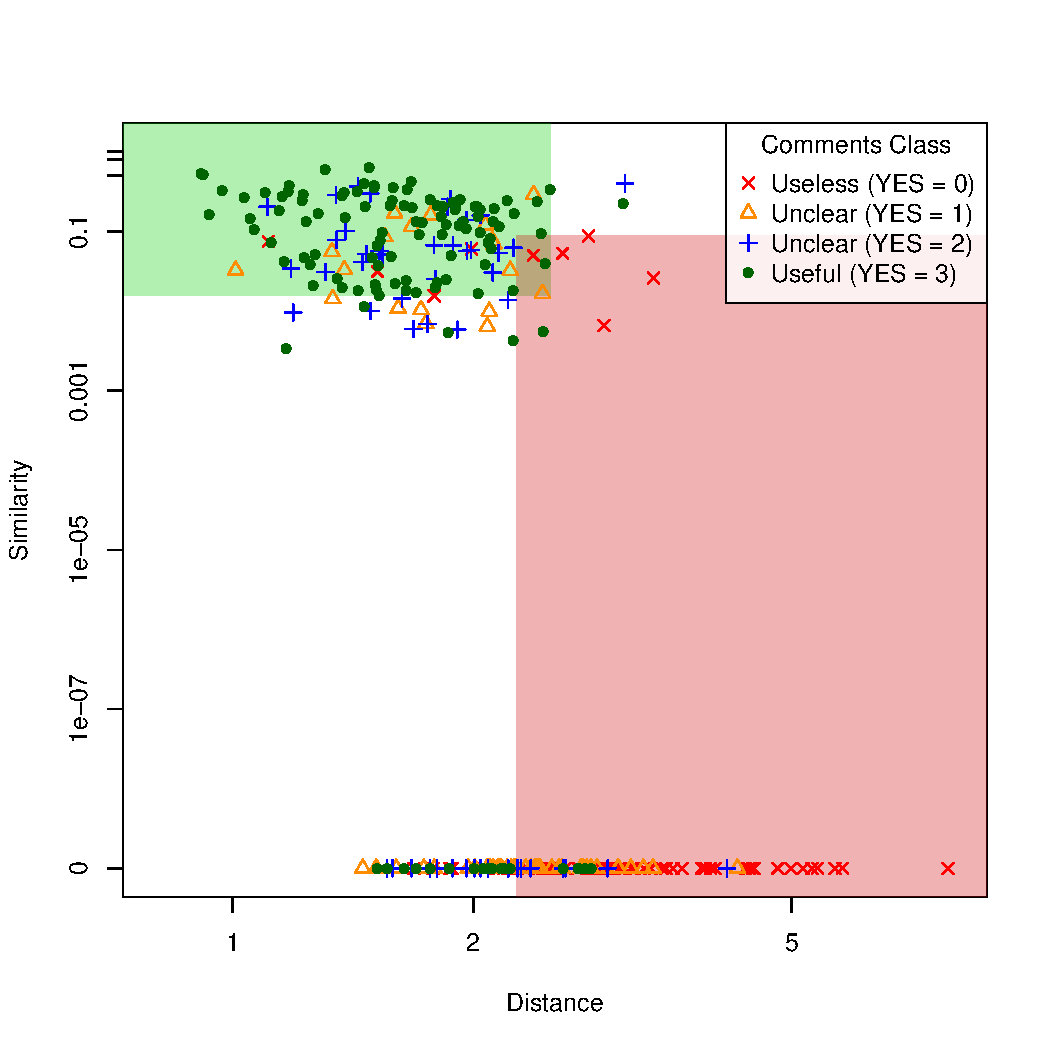
\includegraphics[scale=0.45, trim=0 0 30 50, clip=true]{scatter_log}
\caption{The similarity and distance plot of the training data.
The symbol represents the score, which ranges from 0 to 3.
The green area represents the \emph{useful} classification model and the red area represents the \emph{useless} model.}
\label{fig:scatter}
\end{figure}

To answer this question, we randomly sampled 318 comments from our data set and manually identified usefulness.
Then, we used these comments for both the training and test data set for our approach to determine its effectiveness.
We also determined the effectiveness of our approach using bootstrapping cross validation.

% \dan{What what the effort in person-hours for this?}
% Thai sez:  Average time per comment is 28 seconds.
%            Since we do a lot of other things while training, it gives us a STDEV of 45 seconds.
%            The median, by the way, is just 10 seconds.

% Since our models do not include unclear type of comments, we defined them as negative condition i.e useless comments in case of useful classification (when using $\Theta(c,S_T,D_T)$ model) and useful comments in case of useless classification (when using $\Omega(c,S'_T,D'_T)$ model).
%\dan{I thought we changed this! It would be bad if we didn't. Let me know what the actual situation is here.}
%
% Thai sez:  We did not. Maybe this is just a matter of wording. I believe what the text says is:
%                - For useful classification, we only look for 3 scored comments.
%                - For useless classification, we only look for 0 scored comments.

To determine similarity and dissimilarity thresholds for useful and useless model, we iterated $s_t$ and $d_t$ values from every unique similarity and dissimilarity values in our data set.
%Table \ref{tb:thresholds} shows 5 sets of thresholds that best classify useful and useless comments based on F$_1$ score.
We selected the thresholds that best classify useful and useless comments based on F-measure score and applied models.
The selected models are $\Theta(c,S_T=0.015529,D_T=2.494944)$ for useful comments, and $\Omega(c,S'_T=0.087522,D'_T=2.265679)$ for useless comments.




\textbf{Model Effectiveness Results:} From 318 samples, the comment sets from manual assessment were 85, 111, and 122 for useless set (\texttt{YES} = 0), unclear sets (\texttt{YES} = 1 or 2), and useful set (\texttt{YES} = 3), respectively. The precision and Recall of the models were 0.701 and 0.787 for useful model and 0.648 and 0.824 for useless model. 

Figure \ref{fig:scatter} shows the relationship between usefulness class from our classification model and comment sets from manual assessment. 
The green area represents the \emph{useful} classification model and the red area represents the \emph{useless} classification model. The comments drawn in the green area are those satisfied condition of useful model, and the comments drawn in the red area are those satisfied condition of useless, while the comments drawn in the white area are those not satisfied any condition (i.e. \emph{undetermined}). 
The total number of comments from this classification results is described in Table \ref{tb:classify_number}. 



%%Interpret: comments & model%%%%
Corresponding to the precision and recall values, the figure shows that the majority of comments drawn in green area are comments from the useful set, and very few comments of useless set drawn in this area.
Similarly, majority of comments drawn in the red area are comments from the useless set.
It also shows that the similarity and dissimilarity values of comments in each set are not different from other comments in the same set.
Most comments from the useful set (\texttt{YES} = 3) adhere in the top left of the graph
while those from the useless set (\texttt{YES} = 0) adhere in the bottom right of the graph.
However, the unclear set still spread out over the graph.
Therefore, we cannot determine relationship between their similarity values.

There is an overlap section as shown in Fig. \ref{fig:scatter}.
This is a conflict results between our two models where a comment received true outcome from both classification models.  
This is phenomenon can occur since similarity and dissimilarity values of each group are vague and both  models tend to maximize coverage of classification.
However, from the results in Table \ref{tb:classify_number}, only three comments were selected by both models (overlap). This is very small error for our models.
Excluding the overlap classification result, we can calculate precision and recall as described in Table \ref{tb:classify_number}. Furthermore, there are 12 useless comments (14\%) and 21 useful comments (17\%) still are undetermined (drawn in white area). These comments were not satisfied our models. This suggests us that other indicators are needed to investigate for usefulness classification.

%From the example comment, it shows that these comments discussed on \TODO{insert topic}, but did not contain any word in common.

\begin{table}[!t]
\centering

\caption{Number of comments classified by our approach against ground truth data}
\begin{tabular}{cccccc}
\hline
Result from & \multicolumn{4}{c}{Results from manual assessment}  & \multirow{3}{*}{Precision}\\ \cline{2-5}
Classification &  Useless  & Unclear  & Unclear & Useful \\
Models&  (\texttt{YES}=0) & (\texttt{YES}=1) & (\texttt{YES}=2) & (\texttt{YES}=3) \\
\hline \hline
Useful Class & 3 & 12 & 24 & 95 & 0.709\\
Useless Class & 69 & 23 & 7 & 6 &  0.657\\
Overlap & 1 & 1 & 0 & 1 & - \\
Undetermined & 12 & 24 & 20 & 20 & - \\
\hline
Recall & 0.812 & - & - & 0.778\\ \hline 
\end{tabular}
\label{tb:classify_number}
\end{table}


%\begin{table*}[!t]
%\caption{An accuracy of similarity and dissimilarity thresholds for useful and useless comment classifications}
%\small
%\centering
%\def\arraystretch{1.2}
%\begin{tabular}{ccccccc}
%\hline
%Prediction Models  & Rank & $s_t$ & $d_t$ & F-measure & Precision & Recall \\ \hline \hline
%\multirow{5}{*}{\textbf{useful}: $\Theta(c,S_T=s_t,D_T=d_t)$}
%& 1 & 0.015529 & 2.494944 & 0.741 & 0.701 & 0.787 \\ \cline{2-7}
%& 2 & 0.015529 & 3.077129 & 0.740 & 0.693 & 0.795 \\ \cline{2-7}
%& 3 & 0.016713 & 2.494944 & 0.739 & 0.704 & 0.779 \\ \cline{2-7}
%& 4 & 0.015411 & 2.494944 & 0.738 & 0.696 & 0.787 \\ \cline{2-7}
%& 5 & 0.015411 & 3.077129 & 0.738 & 0.688 & 0.795
%% \\ \cline{2-7}
%% & \multicolumn{3}{r}{Average} &  1.00 & 1.00 & 1.00 \\ \cline{2-7}
%%& \multicolumn{3}{r}{Min-Max} &   1.00 - 1.00 & 1.00 - 1.00  & 1.00 - 1.00
%\\ \hline \hline
%\multirow{5}{*}{\textbf{useless}: $\Omega(c,S'_T=s_t,D'_T=d_t)$}
%& 1 & 0.087522 & 2.265679 & 0.725 & 0.648 & 0.824 \\ \cline{2-7}
%& 2 & 0.087522 & 2.250422 & 0.722 & 0.642 & 0.824 \\ \cline{2-7}
%& 3 & 0.087522 & 2.324771 & 0.720 & 0.663 & 0.788 \\ \cline{2-7}
%& 4 & 0.052856 & 2.265679 & 0.719 & 0.645 & 0.812 \\ \cline{2-7}
%& 5 & 0.087522 & 2.249675 & 0.718 & 0.636 & 0.824
%% \\ \cline{2-7}
%%& \multicolumn{3}{r}{Average} &  1.00 & 1.00 & 1.00 \\ \cline{2-7}
%%& \multicolumn{3}{r}{Min-Max} &   1.00 - 1.00 & 1.00 - 1.00  & 1.00 - 1.00
%\\ \hline
%\end{tabular}
%\label{tb:thresholds}
%\end{table*}

\begin{table*}[!t]
\caption{Results from bootstrapping cross validation of our classification models against random models}
\small
\centering
\def\arraystretch{1.2}
\begin{tabular}{cccc|cc|cc|cc}
\hline
\multicolumn{2}{c}{Classifcation}   & \multicolumn{2}{c|}{Precision} & \multicolumn{2}{c|}{Recall} & \multicolumn{2}{c|}{F-measure} & \multicolumn{2}{c}{Accuracy} \\ \cline{3-10}
\multicolumn{2}{c}{Models} & Avg. & STD. & Avg. & STD. & Avg. & STD. & Avg. & STD. \\ \hline \hline
\multirow{2}{*}{Useful} & $\Theta(c,S_T,D_T)$    &  0.654 & 0.116 &  0.759 & 0.123 & 0.693 & 0.089 & 0.752 & 0.067 \\ \cline{2-10}
& Random     &  0.421 & 0.114 &  0.376 & 0.116 & 0.496 & 0.144 & 0.496 & 0.089 \\ \hline
\multirow{2}{*}{Useless}  & $\Omega(c,S'_T,D'_T)$  &  0.636 & 0.144 &  0.755 & 0.148 & 0.681 & 0.118 & 0.815 & 0.064 \\ \cline{2-10}
& Random    &  0.336 & 0.131 &  0.269 & 0.115 & 0.478 & 0.182 & 0.500 & 0.089 \\
\hline
\end{tabular}
\label{tb:xvalidate}
\end{table*}


\textbf{Validation:}
We validated our approach using bootstrapping cross validation.
We randomly selected 90\% of 318 comments for training set and determine thresholds.
The constructed model is then applied on the remaining 10\% comments as the validation set.
The precision, recall and F-measure scores are measured and recorded.
This validation was repeated 300 times to give an average performance of our models.
For a baseline, we also determined the performance of the random classifier using the same methods.

Table \ref{tb:xvalidate} describes the performance of useful and useless classification models including an average and standard deviation of precision, recall, and F-measure.
The results show that both of our models can achieve 60\% of precision and 75\% of recall, approximately.
In addition, our models also achieved higher results than the random models twice for both precision and recall.


%\begin{table*}[!t]
%\caption{An accuracy of similarity and dissimilarity thresholds for useful and useless comment classifications}
%\small
%\centering
%\def\arraystretch{1.2}
%\begin{tabular}{ccccccc}
%\hline
%Prediction Models & $s_t$ & $d_t$ & F-measure & Precision & Recall \\ \hline \hline
%$\Theta(c,S_T=s_t,D_T=d_t)$   & 0.015529 & 2.494944 & 0.741 & 0.701 & 0.787 \\ \hline
%$\Omega(c,S'_T=s_t,D'_T=d_t)$ & 0.087522 & 2.265679 & 0.725 & 0.648 & 0.824 \\ \hline
%\end{tabular}
%\label{tb:thresholds}
%\end{table*}




According to the results, we can answer RQ1 that \emph{using semantic similarity values as indicators, our approach successfully classify comment usefulness with precision of 0.6 and recall of 0.7 approximately and this is better than random  classification models as twice.}

%After we performed cross validation, we obtained the following result:
%for positive and negative classifications,
%we obtained an average F$_1$ score of 0.693 and 0.681,
%with standard deviation of 0.090 and 0.118, respectively.
%This indicates that we can use our approach to classify with confident of 69.8\%.

%After the similarity and distance metrics have been calculated,
%these metrics appear to be able to separate the useful comments from the non-useful ones,
%as can be seen in Fig.\ref{fig:scatter}.
%Note that many comments have a cosine similarity metric of 0.
%This is because the comment text and the corresponding commit message has no word in comment.






\begin{ResearchQuestions}
\item[RQ2:] Is semantic similarity classification cost-efficient, assurable, and scalable?
\end{ResearchQuestions}

Automatic systems are generally known for saving human effort and also reduce human errors.
We analyze the results to determine the performance of our models.
In addition, we also consider scalability of our models as it only validated in the small set of comments.
% \pick{Trying to explain why we considering this}

\textbf{Cost Efficiency:}
% briefly explain
We determined cost efficiency in terms of time use for manual assessment.
For 318 comments in RQ1, we found that the manual assessment took 7.42 person hours on average.
However, this time can be inaccurate since practitioners did not assess under the controlled environment.

% nitty-gritty details
To be more precise, we considered only the time interval between two votes that are not more than 10 minutes apart.
The average time interval between votes is 28 seconds.
Thus, for 318 comments, the assessment time should be 7.42 person hours.
Using the same average interval time for all 10,583 comments,
we can imply that the manual assessment time would be 82.3 person hours.

% how our model helps
When applying our approach to classify these all comments, the models left only 23.5\% of comments for manual assessment (undetermined comments) as shown in Table \ref{tb:percent}.
This means that only 19.34 person hours of additional manual assessment of these undermined comments are needed, thus saving 76.5\% of human effort.

%To answer this question, timestamps are recorded as three people voted on each comment.
%Since three people work in their leisure time, there is much variability in the time between each vote.
%Therefore, we ignored the time interval between two votes if they are more than 10 minutes apart.
%
%On average, it takes 28 seconds to assess each comment.
%However, the median is 10 seconds, suggesting that most comments take only a little amount of time to assess, while only few comments take long time.
%This also suggests that the time to assess each comment is not normally distributed.
%The standard deviation is 45 seconds.
%
%To estimate the total time for us to assess these 318 comments,
%we multiplied the average time by the number of comments and the number of people.
%This results in 7.42 person hours.
%
%However, to manually assess all 10,583 comments---even with only one person---this would take 82.3 person hours.
%By running our model through all 10,583 comments, only 2,487 comments receive undetermined result.
%That means that about 77\% of the effort is saved.

\textbf{Assurance:} In Table \ref{tb:classify_number}, there are 88\% of useful class have comments with \texttt{YES} = 2 and 3 voting scores. The classification of useless class also have similar proportion i.e. having high number of comment with \texttt{YES} = 0 and 1 voting scores. We conjecture that the unclear comments with \texttt{YES} = 2 might actually be useful comments and comments with \texttt{YES} = 1 might actually be useless. The unclear result could be from error of manual assessment caused by human.
To verify this conjecture, we asked practitioners to re-examine the unclear comments.
We found that 17\% of these 66 comments became unclear because of human error.
This shows that our model \thai{what can we say about this model?}

%As the manual classification can be subjective, these comments were not received three voting scores.  



\textbf{Scalability:} Applying our classification model to all comments results in the proportions shown in Table \ref{tb:percent}.
As the table shows, the proportions are very similar in both the training dataset and all dataset,
which may suggest that our model will have a similar performance in the real data.

\begin{table}[!t]
\caption{Percentage of classifications results for all comments in the \texttt{qtbase} project }
\small
\centering
\def\arraystretch{1.2}
\begin{tabular}{c|c|c}
\hline

Result from & Sample Comments   &  All Comments \\ \cline{2-3}
Classification Models &  318 comments  & 10,583 comments \\ \hline \hline
Useful Class  & 41.8\% & 42.8\% \\
Useless Class   & 33.1\%  & 33.7\% \\
undetermined  & 25.1\% & 23.5\% \\ \hline
\end{tabular}
\label{tb:percent}
\end{table}

%\pick{Note from Dan sensei,}
%For cpost effectivness we can state the reduction percentage in the number of comments that much be checked manually.
% Also point out how much effort manual classification takes and that it is error prone (probably mor so than the automated method!
%You cannot, but some estimates are possble
%first, human beings have a fairly well known rate of making errors in classification
%second, look at the comments in the training set that the method classified differently, especially the unclear.
%Review these to see if the method suggested a better classification than was originally made by the assessors
%You can consider these errors. Now look at what wans the percent of errors in the training set
%This is also an estimate of the human error rate




% !TEX root = ../paper.tex
\section{Discussion}
Our results have shown that our semantic similarity is practical to assist in reducing effort and error proneness of manual assessment of comment usefulness.  
Besides this result, we also found some noteworthy findings in our case study:

% tuning the F score for precision and recall
%Depending on the use case, we can fine-tune the F-score to give more weight to recall or precision.
%For instance, if we wanted to measure the amount of useful comments within a large dataset, more weight can be given to precision, sacrificing some useful comments.
%If we wanted to modify a code review software such that it displays useful comments more prominently, more weight can be given to recall.

% examples.
\subsection{What kind of comments cannot be classified using semantic similarity?}

From the results of RQ1, we found that some comments were not determined by our model.
Specifically, we were interested in why some manually assessed useful comments (\texttt{YES} = 3) and useless comments (\texttt{YES} = 0) were undetermined.
To investigate the reason behind this, we reviewed these comments and the corresponding commit messages.
We found that there were few common keywords between the comments and commit messages and their lengths are relatively unequal.
This makes for low similarity values and low dissimilarity values as shown in bottom left white area in Fig. \ref{fig:scatter}. There simply isn't enough semantic information to determine anything.


%In some cases, similarity and dissimilarity failed to measure the usefulness of the comment,
%due to the same word being used in a different context.
%For example, consider this excerpt from the commit message: \emph{``In the no-assert case, make Q\_ASSERT decay to Q\_ASSUME. I can confirm
%better code generation with GCC at least.''}
%This comment, \emph{``I'll study the generated code a bit more,''} is just an author's response, and thus is not technically contributing. However, it is classified as a useful comment. This may be caused by the word \emph{generate} which appears in both documents.


%\subsection{Binary Classification}
%\subsection{How much impact of unclear class on model construction?}
%\pick{This topic of discuss should be changed....}
% % noisy data, and binary classification
%
% 
% 
%Our training data contains much variability because there are disagreements between our judgment of ``usefulness,'' rendering our results unclear; they cannot be classified as either useful or not useful.
%This impacts the trade-off between the precision and recall for our model, and consequently, the F$_1$ score.
%
%Another approach we tried is to perform a \emph{binary classification}.
%This means we assume that there are no unclear or undetermined comments; only useful and useless.
%For this, we removed the samples with 1 and 2 \texttt{YES} votes from our training set.
%This leaves us with 209 remaining samples, all without a disagreement.
%By performing cross-validation using these samples, we obtained a much better F$_1$ score of 0.896.
%
%However, we could not objectively measure the F$_1$ score for all samples, because giving positive or negative classification to 1 and 2-scored samples introduces a bias.
%But interestingly, the results seen in Fig.\ref{fig:binary} suggests that the binary classifier tends to gives positive classification to samples with score of 2 more than samples with score of 1, and the \emph{vice versa} for negative classification. 
%
%\begin{figure}[h]
%\centering
%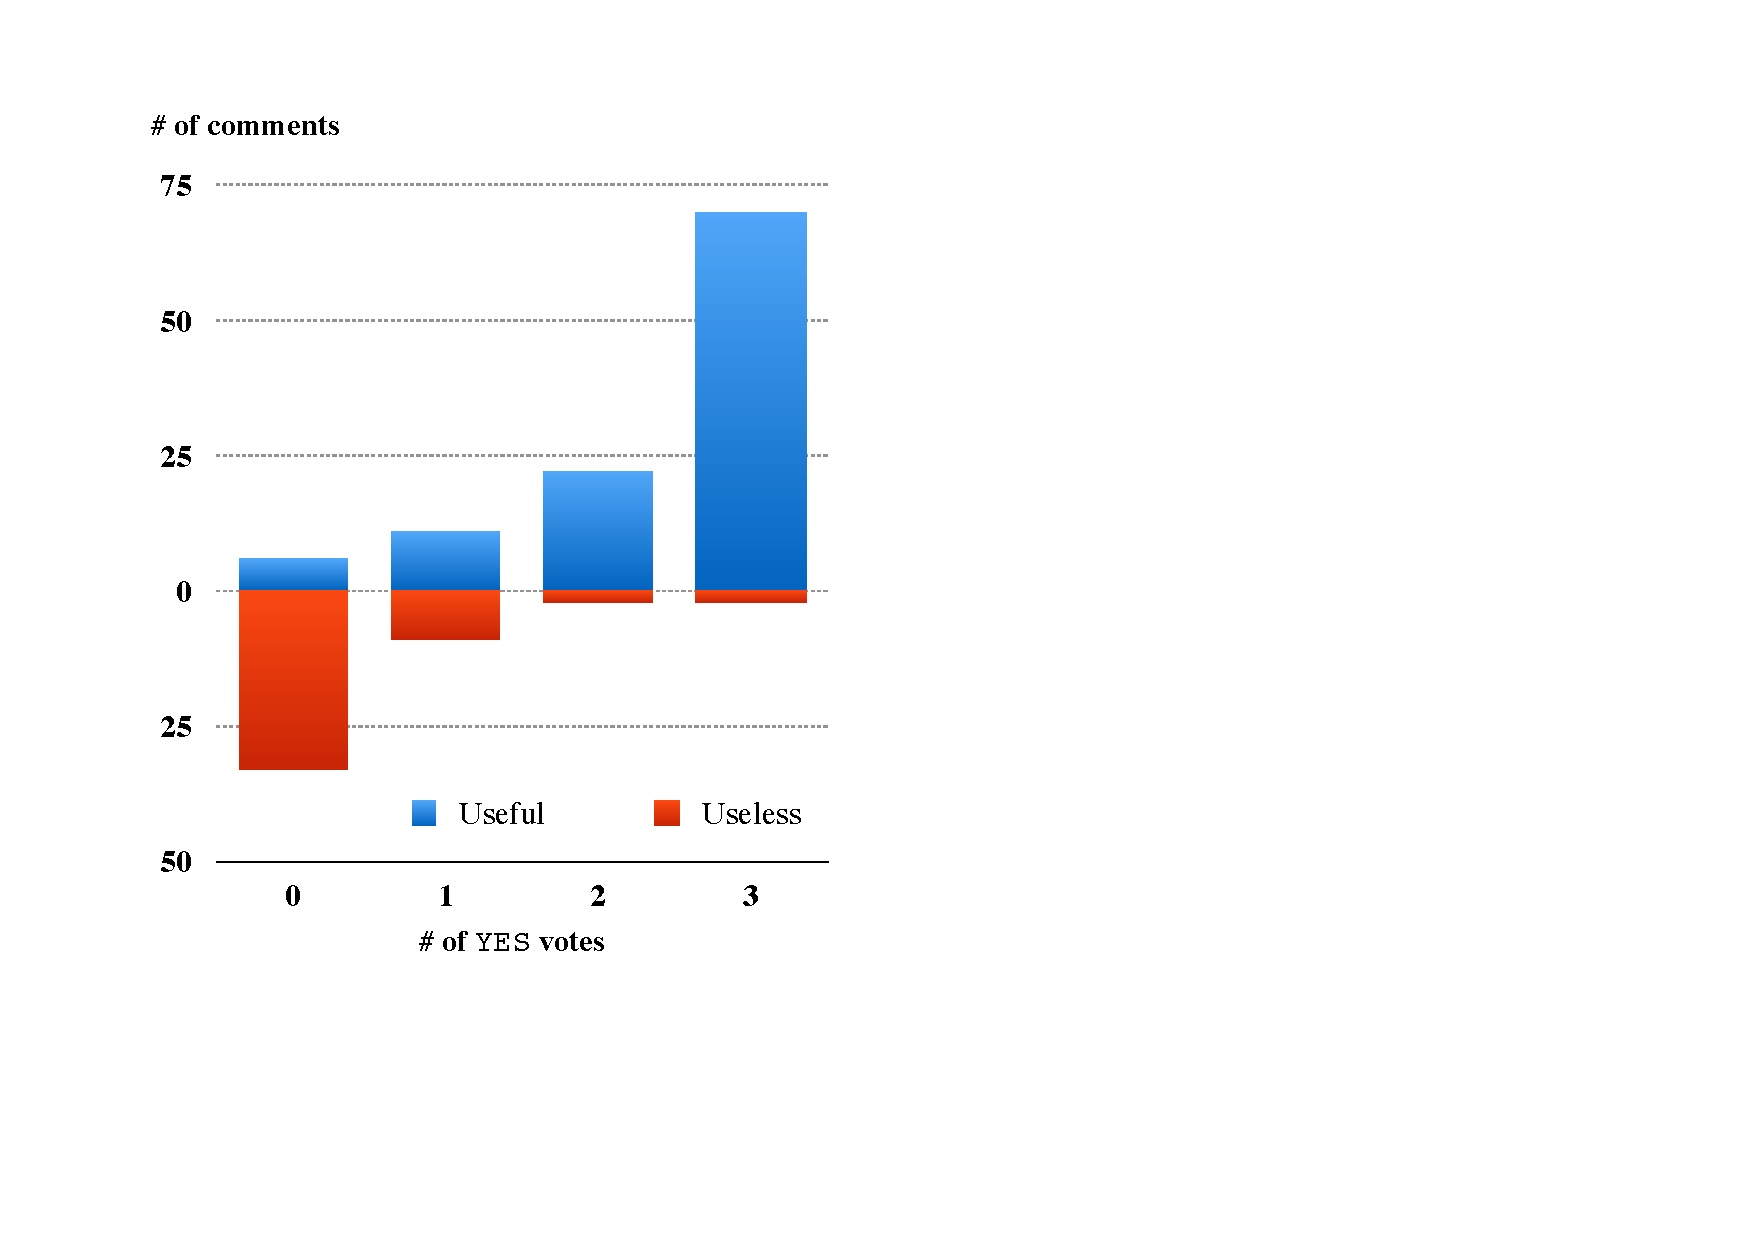
\includegraphics[width=2.5in]{posneg}
%\caption{The amount of comments by score classified by the binary classifier.}
%\label{fig:binary}
%\end{figure}

\subsection{Can other text mining techniques be used to classify discussions?}
To find relevance between comments and the corresponding commit message,
topic modeling technique can be used, as the study of \cite{Barua2012a}.
This technique discovers topics for a given collection of documents.
However, in MCR context, the documents generally are very short statements and discussions, which makes it unsuitable for LDA. 
Nevertheless, we have tried applying Latent Dirichlet Allocation (LDA, a well-known topic modeling technique) model on our data set.
As expected, LDA generated ambiguous topics with many unrelated keywords. Again, as discussed above, there is simply not enough information since the content of the documents are too short, and thus is insufficient for LDA to correctly determine the topic. Others techniques could be investigated in the future to improve results.

%\subsection{Reasons of Classification}
% reasons for classification as useful or not useful
\subsection{What decisions are made during the manual classification?}
During manual comment usefulness assessment, we recorded the participants' rationale to verify that the comments actually direct contribute to the proposed changes. We can summarize that most of reasons for \texttt{YES} voting are: the comments 1) contain new information 2) contain constructive suggestions, 3) discuss directly to the proposed changes, and 4) discuss specific technical matters. For \texttt{NO} voting, we can summarize that the comments 1) are chatting (just communication), 2) talking about matters unrelated to the proposed changes, 3) discuss about process workflow and supporting system (e.g. Git and Gerrit).
%During the training process, reasons for the judgment are recorded. Examples of reasons for positive comments include:
%
%\begin{itemize}
%	\item they contain new information;
%	\item they contain constructive suggestions;
%	\item they discuss directly about the change; and
%	\item they discuss technical matters.
%\end{itemize}
%
%Examples of reasons for negative comments include:
%
%\begin{itemize}
%	\item chatting (i.e. no new information, just communication);
%	\item not discussing directly about the change;
%	\item discussing about the process workflow; and
%	\item discussing about Git or Gerrit itself.
%\end{itemize}

\subsection{Can the determined thresholds in this study be used to other projects?}

In this study, we determined the similarity conditions using a training set from the Qt project and the results show that the conditions can indeed classify usefulness of comments.
However, we have no basis for believing that the threshold values obtained for one project would apply equally well for another project. To apply our approach on other projects, a new training set is still required which implies additional manual assessment.
This limits the practicality of application our our method to projects with a large enough number of comments, where the classification effort saved overcomes the training costs.
To fully automate this approach, we have to investigate the use of similarity conditions for many other different projects. Thus, additional studies are needed to improve our approach and potentially identify invariant conditions for similarly and usefulness. 

%
%Secondly, owing to the subjective assessment of usefulness, this representation fundamentally implies supervised classification requiring nontrivial training data to define representative classification sets. This decreases the cost-effectiveness and limits the practicality of application to projects with a large enough number of comments, where the classification effort saved overcomes the training costs.






\section{Threat to Validity}


\section{Conclusion and Future Work}


\IEEEpeerreviewmaketitle

\bibliographystyle{IEEEtran}

\bibliography{references}



% that's all folks
\end{document}


